\documentclass[../Main.tex]{subfiles}
\begin{document}
En el siglo XX, las teorías que explicaban el comportamiento de la naturaleza comenzaron a cambiar radicalmente. La no invarianza de las ecuaciones de Maxwell bajo las transformaciones de Galileo y  el nulo resultado del experimento de Michelson-Morley en detectar el ether---entidad en la que se propagaría la luz---, llevó a Albert Einstein a la formulación de la Relatividad Especial en 1905, pudiendo así explicar fenómenos a velocidades cercanas a las de la luz, introduciendo el concepto de espacio-tiempo. No obstante, su mayor invención llegaría en 1915 cuando introdujo la teoría de la Relatividad General. Esta nueva teoría de gravedad cumpliría con 3 principios generales: primero, sus ecuaciones son tensoriales, por lo tanto covariantes ante transformaciones de coordenadas. Además, en esta formulación, el espacio-tiempo es dinámico y no un escenario inmóvil en donde suceden las cosas. Segundo, involucran hasta segundas derivadas de la métrica, lo que las hace compatibles con las ecuaciones de movimiento que conocemos en las teorías clásicas de la física. Finalmente, como tercera propiedad, estas ecuaciones recuperan la gravedad de Newton en el llamado límite de bajas velocidades y campo débil. Siguiendo un procedimiento puramente físico, Einstein logro escribir las ecuaciones de campo de la Relatividad General, estas son
\begin{equation}\label{eomeinstein}
    R_{\mu\nu}-\frac{1}{2}g_{\mu\nu}R =\frac{8\pi G}{c^4}T_{\mu\nu}\, ,
\end{equation}
donde $R_{\mu\nu}$ es el tensor de Ricci, $g_{\mu\nu}$ es el tensor métrico, $g^{\mu\nu}R_{\mu\nu}=R$ es el escalar de Ricci y $T_{\mu\nu}$ es el tensor de energía-momentum de la materia. Estas ecuaciones han logrado describir satisfactoriamente fenómenos que hasta el momento no eran posibles de explicar con la teoría de gravitación universal de Newton, tales como la precesión del perihelio de Mercurio, deflexión de la luz por el sol, el redshift gravitacional de la luz, entre otros \cite{Will:2014kxa}. 





\section{Acción de Einstein-Hilbert y ecuaciones de movimiento}
Paralelamente a Einstein, David Hilbert trabajaba en obtener las Eqs.~\eqref{eomeinstein} de un principio variacional. Para ello, propuso un funcional de la métrica sobre una variedad diferencial $\mathcal{M}$ que fuera invariante bajo transformaciones de coordenadas y que entregara las ecuaciones~\eqref{eomeinstein} al realizar variaciones arbitrarias con respecto de los campos dinámicos. A este principio de acción hoy lo conocemos como acción de Einstein-Hilbert, la cual está dada por
\begin{equation}\label{EHM}
    I[g_{\mu\nu},\psi]=\kappa \int_{\mathcal{M}} d^{4}x \sqrt{\lvert g\rvert}\, R + \int_{\mathcal{M}}d^{4}x \sqrt{\lvert g\rvert}\, \Lag_M[g_{\mu\nu},\psi] \, , 
\end{equation}
en donde $\psi$ es algún campo de materia, $\kappa=(16\pi G)^{-1}$ con $G$ la constante de Newton, $g=\det g_{\mu\nu}$ es el determinante de la métrica, y $\Lag_M$ es un Lagrangiano de materia, cuya variación con respecto de sus campos dinámicos entrega las ecuaciones de movimiento para la materia. Por otro lado, la variación de $\Lag_M$ con respecto de la métrica entrega el tensor de energía-momentum definido por
\begin{align}
T_{\mu\nu} = -\frac{2}{\sqrt{|g|}}\frac{\delta}{\delta g^{\mu\nu}}\left(\sqrt{|g|}\,\Lag_M\right)\,.
\end{align}
En esta sección, vamos a considerar la acción \eqref{EHM} sin materia, i.e. $\Lag_{M}=0$ La variación arbitraria de esta acción con respecto de la métrica entrega
\begin{align} \notag
     \delta I[g_{\mu\nu}]&=\kappa \int_{\mathcal{M}} d^{4}x \delta[\sqrt{\lvert g\rvert}\, R]\\
     &=\kappa \int_{\mathcal{M}} d^{4}x \left[\delta(\sqrt{\lvert g\rvert})R\,+ \sqrt{\lvert g\rvert}\delta R\right] \, . \label{variacion1}
\end{align}
Analicemos el primer termino de Ec.~\eqref{variacion1}. Conocemos que la variación cumple con la regla de Leibniz, por lo que se tiene
\begin{align} \notag
    \delta\sqrt{\lvert g \rvert}&=\frac{1}{2}\frac{1}{\sqrt{\lvert g \rvert}}\delta \lvert g \rvert\\ \notag
    &=\frac{1}{2}\lvert g \rvert^{-\frac{1}{2}}g^{\mu\nu}\delta g_{\mu\nu}\lvert g \rvert \\ \notag
    &=\frac{1}{2}\sqrt{\lvert g \rvert}g^{\mu\nu}\delta g_{\mu\nu} \, \\ 
    &=-\frac{1}{2}\sqrt{\lvert g \rvert}g_{\mu\nu}\delta g^{\mu\nu} \, ,\label{vd}
\end{align}
en donde para la variación del determinante de la métrica hemos usado la fórmula de Jacobi
\begin{align*}
    \delta \lvert g \rvert=\delta\left(e^{\Tr[\log(g_{\mu\nu})]}\right)&=\delta\left(\Tr[\log(g_{\mu\nu})]\right)e^{\Tr[\log(g_{\mu\nu})]}\\
    &=\Tr[\delta\left(\log(g_{\mu\nu})\right)]e^{\Tr[\log(g_{\mu\nu})]}\\
    &=\Tr\left(g^{\mu\nu}\delta g_{\mu\nu}\right)e^{\Tr[\log(g_{\mu\nu})]}\\
    &=g^{\mu\nu}\delta g_{\mu\nu}\lvert g \rvert \, ,
\end{align*}
en donde se puede ver que, en la penúltima linea, hemos tomado la traza al elemento dentro del paréntesis. Además, en la Ec.~\eqref{vd} usamos la propiedad 
\begin{align}
    \delta(g_{\mu\nu}g^{\nu\alpha})=0\, .
\end{align}
Estudiemos ahora la variación del termino $\delta R$. Comencemos por la definición del escalar de Ricci
\begin{equation} \label{varr}
    \delta R= \delta (g^{\mu\nu}R_{\mu\nu})=\delta (g^{\mu\nu}R^{\lambda}\,_{\mu\lambda\nu})=\delta g^{\mu\nu}R^{\lambda}_{\ \mu\lambda\nu}+g^{\mu\nu}\delta R^{\lambda}_{\ \mu\lambda\nu} \, .
\end{equation}
Para obtener la variación del tensor de Ricci vamos a considerar su definición 
\begin{equation}
R^{\lambda}_{\ \rho\mu\nu}=\partial_{\mu}\Gamma^{\lambda}_{\rho\nu}-\partial_{\nu}\Gamma^{\lambda}_{\rho\mu}+\Gamma^{\lambda}_{\sigma\mu}\Gamma^{\sigma}_{\rho\nu}-\Gamma^{\lambda}_{\sigma\nu}\Gamma^{\sigma}_{\rho\mu}\, ,
\end{equation}
en donde $\Gamma^{\lambda}_{\lambda\mu}$ es el símbolo de Christoffel que está dado por
\begin{equation} \label{chr}
    \Gamma^{\lambda}_{\mu\nu}=\frac{1}{2}g^{\lambda\gamma}\left(\partial_{\mu}g_{\gamma\nu}+\partial_{\nu}g_{\mu\gamma}-\partial_{\gamma}g_{\mu\nu}\right)\,.
\end{equation}
Luego, variando el tensor de Riemann obtenemos
\begin{align} \notag
\delta R^{\lambda}_{\ \rho\mu\nu}&=\delta(\partial_{\mu}\Gamma^{\lambda}_{\rho\nu})-\delta(\partial_{\nu}\Gamma^{\lambda}_{\rho\mu})+\delta(\Gamma^{\lambda}_{\sigma\mu}\Gamma^{\sigma}_{\rho\nu})-\delta(\Gamma^{\lambda}_{\sigma\nu}\Gamma^{\sigma}_{\rho\mu})\\
&=\partial_{\mu}\delta\Gamma^{\lambda}_{\rho\nu}-\partial_{\nu}\delta\Gamma^{\lambda}_{\rho\mu}+\delta(\Gamma^{\lambda}_{\sigma\mu})\Gamma^{\sigma}_{\rho\nu}+\Gamma^{\lambda}_{\sigma\mu}\delta(\Gamma^{\sigma}_{\rho\nu})-\delta(\Gamma^{\lambda}_{\sigma\nu})\Gamma^{\sigma}_{\rho\mu}-\Gamma^{\lambda}_{\sigma\nu}\delta(\Gamma^{\sigma}_{\rho\mu})\, ,
\end{align}
en donde usamos que la variación conmuta con las derivadas parciales. Ahora, se puede ver que es posible armar derivadas covariantes del siguiente modo
\begin{align}\notag
    \nabla_{\mu}(\delta\Gamma^{\lambda}_{\rho\nu})&= \partial_{\mu}(\delta\Gamma^{\lambda}_{\rho\nu})+\Gamma^{\lambda}_{\mu\sigma}(\delta\Gamma^{\sigma}_{\rho\nu})-\Gamma^{\sigma}_{\mu\rho}(\delta\Gamma^{\lambda}_{\sigma\nu})-\Gamma^{\sigma}_{\mu\nu}(\delta\Gamma^{\lambda}_{\rho\sigma})\, ,\\
    \nabla_{\nu}(\delta\Gamma^{\lambda}_{\rho\mu})&= \partial_{\nu}(\delta\Gamma^{\lambda}_{\rho\mu})+\Gamma^{\lambda}_{\nu\sigma}(\delta\Gamma^{\sigma}_{\rho\mu})-\Gamma^{\sigma}_{\nu\rho}(\delta\Gamma^{\lambda}_{\sigma\mu})-\Gamma^{\sigma}_{\nu\mu}(\delta\Gamma^{\lambda}_{\rho\sigma})\, .
\end{align}
Reemplazando las expresiones de las derivadas parciales en la variación del tensor de Riemann, encontramos que 
\begin{eqnarray*}
    \delta R^{\lambda}_{\ \rho\mu\nu}&=&\nabla_{\mu}(\delta\Gamma^{\lambda}_{\rho\nu})-\Gamma^{\lambda}_{\mu\sigma}(\delta\Gamma^{\sigma}_{\rho\nu})+\Gamma^{\sigma}_{\mu\rho}(\delta\Gamma^{\lambda}_{\sigma\nu})+\Gamma^{\sigma}_{\mu\nu}(\delta\Gamma^{\lambda}_{\rho\sigma})\\
    &-&\nabla_{\nu}(\delta\Gamma^{\lambda}_{\rho\mu})+\Gamma^{\lambda}_{\nu\sigma}(\delta\Gamma^{\sigma}_{\rho\mu})-\Gamma^{\sigma}_{\nu\rho}(\delta\Gamma^{\lambda}_{\sigma\mu})-\Gamma^{\sigma}_{\nu\mu}(\delta\Gamma^{\lambda}_{\rho\sigma})\\
     &+&\delta(\Gamma^{\lambda}_{\sigma\mu})\Gamma^{\sigma}_{\rho\nu}+\Gamma^{\lambda}_{\sigma\mu}\delta(\Gamma^{\sigma}_{\rho\nu})-\delta(\Gamma^{\lambda}_{\sigma\nu})\Gamma^{\sigma}_{\rho\mu}-\Gamma^{\lambda}_{\sigma\nu}\delta(\Gamma^{\sigma}_{\rho\mu})\,.
\end{eqnarray*}
Podemos notar que varios términos se cancelan, así nos queda un resultado importante que se conoce como Identidad de Palatini 
\begin{align}
    \delta R^{\lambda}{}_{\rho\mu\nu}=2 \nabla_{[\mu } \delta \Gamma_{\rho \mid \nu]}^\lambda \label{palatini}\, ,
\end{align}
luego si cambiamos $\mu\to\lambda$ nos queda 
\begin{equation}
    \delta R^{\lambda}\,_{\rho\lambda\nu}=\nabla_{\lambda}\delta\Gamma^{\lambda}_{\rho\nu}-\nabla_{\nu}\delta\Gamma^{\lambda}_{\rho\lambda}\, . \label{pal}
\end{equation}
Teniendo como resultado la variación del Riemann en la Ec.~\eqref{pal}, reemplazamos en la variación arbitraria~\eqref{varr} y obtenemos
\begin{align} \nonumber
    \delta R&=\delta g^{\mu\nu}R^{\lambda}\,_{\mu\lambda\nu}+g^{\mu\nu}\delta R^{\lambda}\,_{\mu\lambda\nu}\\ \notag
    &=\delta g^{\mu\nu}R^{\lambda}\,_{\mu\lambda\nu}+g^{\mu\nu}(\nabla_{\lambda}\delta\Gamma^{\lambda}_{\mu\nu}-\nabla_{\nu}\delta\Gamma^{\lambda}_{\mu\lambda})\\
    &=\delta g^{\mu\nu}R^{\lambda}\,_{\mu\lambda\nu}+2g^{\mu\nu}\nabla_{[\lambda}\delta\Gamma^{\lambda}_{\mu|\nu]}\, . \label{varRie}
\end{align}
Reemplazando los resultados de las variaciones de cada termino de la Ec.~\eqref{variacion1} y reordenando nos queda
\begin{align} \nonumber
     \delta I[g_{\mu\nu}]&=\kappa \int_{\mathcal{M}} d^{4}x \left[\left(-\frac{1}{2}\sqrt{\lvert g \rvert}g_{\mu\nu}\,\delta g^{\mu\nu}\right)R\,+ \sqrt{\lvert g\rvert}\left(\delta g^{\mu\nu}R_{\mu\nu}+2g^{\mu\nu}\nabla_{[\lambda}\delta\Gamma^{\lambda}_{\mu|\nu]}\right)\right] \\
     &=\kappa \int_{\mathcal{M}} d^{4}x \sqrt{\lvert g \rvert}\left(R_{\mu\nu}-\frac{1}{2}g_{\mu\nu}R\right)\delta g^{\mu\nu}+2\kappa \int_{\mathcal{M}} d^{4}x \sqrt{\lvert g \rvert}\,g^{\mu\nu}\nabla_{[\lambda}\delta\Gamma^{\lambda}_{\mu|\nu]}\,.
\end{align}
Analicemos el último término de la expresión que obtuvimos. Ahora, nuestro objetivo sera escribirlo como un termino de borde. Antisimetrizar los índices de la derivada covariante es equivalente escribir a la expresión anterior con deltas generalizadas, esto es, 
\begin{align}
2g^{\mu\nu}\nabla_{[\lambda}\delta\Gamma^{\lambda}_{\mu|\nu]}=2\cdot 2g^{\mu\nu}\delta^{[\rho}_{[\lambda}\delta^{\sigma]}_{\nu]}\nabla_{\rho}\delta\Gamma^{\lambda}_{\mu\sigma}\, .
\end{align}
Luego, usando la definición de la delta de Kronecker generalizada,
\begin{equation}
\delta^{\mu_{1}...\mu_{p}}_{\nu_{1}...\nu_{p}}=p!\delta^{[\mu_{1}...\mu_{p}]}_{[\nu_{1}...\nu_{p}]}=p!\delta^{[\mu_{1}...\mu_{p}]}_{\nu_{1}...\nu_{p}}=p!\delta^{\mu_{1}...\mu_{p}}_{[\nu_{1}...\nu_{p}]}\, ,
\end{equation}
nos queda lo siguiente
\begin{align}  \notag  2g^{\mu\nu}\nabla_{[\lambda}\delta\Gamma^{\lambda}_{\mu|\nu]}&=2g^{\mu\nu}\delta^{\rho\sigma}_{\lambda\nu}\nabla_{\rho}\delta\Gamma^{\lambda}_{\mu\sigma}\\ \notag
&=2\nabla_{\rho}\left(g^{\mu\nu}\delta^{\rho\sigma}_{\lambda\nu}\delta\Gamma^{\lambda}_{\mu\sigma}\right)\\
&\equiv 2\nabla_{\mu}\Theta^{\mu}\, ,
    \end{align}
con $\Theta^{\mu}=g^{\mu\nu}\delta^{\rho\sigma}_{\lambda\nu}\delta\Gamma^{\lambda}_{\mu\sigma}$ y donde hemos usado la condición de metricidad $\nabla_{\lambda}g_{\mu\nu}=0$ y que la derivada covariante de la delta generalizada es cero ya que es un tensor constante. Entonces, podemos escribir la variación de la  acción del siguiente modo
\begin{equation}
    \delta I[g_{\mu\nu}]=\kappa \int_{\mathcal{M}} d^{4}x \sqrt{\lvert g \rvert}G_{\mu\nu}\delta g^{\mu\nu}+2\kappa \int_{\mathcal{M}} d^{4}x \sqrt{\lvert g \rvert}\nabla_{\mu}\Theta^{\mu}\,, \label{varinicial}
\end{equation}
con el tensor de Einstein definido como  $G_{\mu\nu}=R_{\mu\nu}-\frac{1}{2}g_{\mu\nu}R$. Finalmente, usando el teorema de Stokes podemos escribir el último término como un término de borde. De este modo, encontramos que
\begin{equation}
    \delta I[g_{\mu\nu}]=\kappa \int_{\mathcal{M}} d^{4}x \sqrt{\lvert g \rvert}G_{\mu\nu}\delta g^{\mu\nu}+2\kappa\sigma \int_{\partial\mathcal{M}} d^{3}x \sqrt{\lvert h \rvert}\Theta^{\mu}n_{\mu}\, , \label{var3}
\end{equation} 
con $h_{\mu\nu}=g_{\mu\nu}-\sigma n_{\mu}n_{\nu}$ la métrica inducida en $\partial_\mathcal{M}$, $n_{\mu}$ el vector normal a una hipersuperficie $\partial\mathcal{M}$ cerrada que puede ser tipo tiempo o tipo espacio y $\sigma=n_{\mu}n^{\mu}=\pm 1$ donde el valor de la norma depende si el vector normal es tipo tiempo ($\sigma=-1$) o tipo espacio ($\sigma=1$). Estos elementos serán vistos con claridad en la Sección que sigue. 

Podemos reducir aún más la Ec.~\eqref{var3}, considerando la condición de metricidad
\begin{align}
\nabla_{\lambda}g_{\mu\nu}=
    \partial_{\lambda}g_{\mu\nu}-\Gamma^{\alpha}_{\mu\lambda}g_{\alpha\nu}-\Gamma^{\alpha}_{\nu\lambda}g_{\mu\alpha}=0\, , \label{met}
\end{align}
y tomando la variación a ambos lados de ésta ecuación. Así, obtenemos
\begin{eqnarray}
    \partial_{\lambda}\delta g_{\mu\nu}-\delta\Gamma^{\alpha}_{\mu\lambda}g_{\alpha\nu}-\Gamma^{\alpha}_{\mu\lambda}\delta g_{\alpha\nu}-\delta\Gamma^{\alpha}_{\nu\lambda}g_{\mu\alpha}-\Gamma^{\alpha}_{\nu\lambda}\delta g_{\mu\alpha}=0 \, .
\end{eqnarray}
Notemos que los primeros tres términos forman la derivada covariante de $\delta g_{\mu\nu}$
\begin{equation}
    \nabla_{\lambda}\delta g_{\mu\nu}=\partial_{\lambda}\delta g_{\mu\nu}-\Gamma^{\alpha}_{\mu\lambda}\delta g_{\alpha\nu}-\Gamma^{\alpha}_{\nu\lambda}\delta g_{\mu\alpha}\label{1} \, .
\end{equation}
Ahora, reemplazando la derivada covariante de la Ec.~\eqref{1} en la variación de la condición de metricidad~\eqref{met} y haciendo permutaciones cíclicas de los índices $\lambda$, $\mu$ y $\nu$, obtenemos
\begin{eqnarray} \label{2}
    \nabla_{\lambda}\delta g_{\mu\nu}&=&\delta\Gamma^{\alpha}_{\mu\lambda}g_{\alpha\nu}+\delta\Gamma^{\alpha}_{\nu\lambda}g_{\mu\alpha} \, ,\\
    \nabla_{\nu}\delta g_{\lambda\mu}&=&\delta\Gamma^{\alpha}_{\lambda\nu}g_{\alpha\mu}+\delta\Gamma^{\alpha}_{\nu\mu}g_{\alpha\lambda}\label{3}\, ,\\ 
    \nabla_{\mu}\delta g_{\nu\lambda}&=&\delta\Gamma^{\alpha}_{\nu\mu}g_{\alpha\lambda}+\delta\Gamma^{\alpha}_{\mu\lambda}g_{\nu\alpha}\label{4} \, .
\end{eqnarray}
Luego, sumamos \eqref{2}, \eqref{3} y restamos \eqref{4}, obteniendo
\begin{eqnarray*}
    \nabla_{\lambda}\delta g_{\mu\nu}+\nabla_{\nu}\delta g_{\lambda\mu}-\nabla_{\mu}\delta g_{\nu\lambda}&=&\cancel{\delta\Gamma^{\alpha}_{\mu\lambda}g_{\alpha\nu}}+\delta\Gamma^{\alpha}_{\lambda\nu}g_{\mu\alpha}+\delta\Gamma^{\alpha}_{\lambda\nu}g_{\alpha\mu}+\cancel{\delta\Gamma^{\alpha}_{\nu\mu}g_{\alpha\lambda}}-\cancel{\delta\Gamma^{\alpha}_{\nu\mu}g_{\alpha\lambda}}-\cancel{\delta\Gamma^{\alpha}_{\mu\lambda}g_{\nu\alpha}}\\
&=&2\delta\Gamma^{\alpha}_{\lambda\nu}g_{\mu\alpha} \, .
\end{eqnarray*}
Multiplicando a ambos lados por $\frac{1}{2}g^{\mu\alpha}$ para despejar la variación del símbolo de Christoffel, nos queda
\begin{equation}
    \delta\Gamma^{\alpha}_{\lambda\nu}=\frac{1}{2}g^{\mu\alpha}\left(\nabla_{\lambda}\delta g_{\mu\nu}+\nabla_{\nu}\delta g_{\lambda\mu}-\nabla_{\mu}\delta g_{\nu\lambda}\right) \, . \label{varchrr}
\end{equation}
Usando el resultado anterior multiplicado por la delta generalizada expandida podemos encontrar que
\begin{equation}
g^{\mu\nu}\delta^{\rho\sigma}_{\lambda\nu}\delta\Gamma^{\lambda}_{\mu\sigma}=\nabla_{\rho}\delta g^{\rho\mu}-g^{\sigma\rho}\nabla^{\mu}\delta g_{\rho\sigma}\,
\end{equation}
finalmente reemplazando esto en la variación de la acción de Einstein-Hilbert \eqref{var3}
\begin{equation}
    \delta I[g_{\mu\nu}] =\kappa\int_{\mathcal{M}}d^{4}x \sqrt{\lvert g\rvert}G_{\mu\nu}\delta g^{\mu\nu}+\kappa\sigma\int_{\partial\mathcal{M}}d^{3}x \sqrt{\lvert h\rvert}\left(\nabla^{\rho}\delta g_{\rho\mu}-g^{\sigma\rho}\nabla_{\mu}\delta g_{\rho\sigma}\right)n^{\mu}\, . \label{varfin}
\end{equation}
Si estudiamos con detenimiento este resultado, nos encontramos con que esta acción no tiene un principio variacional bien definido cuando imponemos condiciones de borde de Dirichlet para la métrica. Esto se debe a que hay términos que dependen tanto como de la derivada de la variación de la métrica y términos que van como la derivada normal de la variación de la métrica. En la siguiente sección veremos como solucionar el problema del principio variacional de la acción de Einstein-Hilbert.




\section{Principio variacional}

Hemos visto que la variación de la acción de Einstein-Hilbert con respecto a la métrica nos entrega la Ec.~\eqref{varfin}. El primer término nos da las ecuaciones de Einstein $G_{\mu\nu}=0$, mientras que la segunda integral es un término de borde. El primer término del paréntesis depende de la variación de la métrica $\delta g_{\mu\nu}$, por lo que al  imponer las condiciones de borde tipo Dirichlet estándar i.e., $\delta g_{\mu\nu}\big|_{\partial\mathcal{M}}=0$ se anula. Sin embargo, el segundo término del paréntesis depende de las derivadas normales de la variación de la métrica, es decir, $n^{\mu}\nabla_{\mu}\delta g_{\rho\sigma}$, por lo que no se hace cero al imponer condiciones de borde tipo Dirichlet. Entonces, podemos concluir que estas condiciones de borde no conducen a un principio variacional bien definido, ya que la variación de la acción no se anula cuando la evaluamos en soluciones a sus ecuaciones de movimiento.
La forma de resolver problema consiste en agregar un término de borde adecuado para la acción. De esta manera, las ecuaciones de movimiento no cambian y para condiciones de borde tipo Dirichlet el término de borde puede ser elegido de forma tal que su variación cancele las derivadas normales que aparecen en la acción. 







\subsection{Interludio: Geometría de hipersuperficies}
Si bien se conoce que la elección de un  término de borde no es único, ya que los términos de borde no cambian las ecuaciones de movimiento, Gibbons, Hawking y York \cite{Gibbons:1976ue,York:1972sj} se dieron cuenta que agregando un término que se construía a partir de la traza de la curvatura extrínseca se cancelaban exactamente las derivadas normales problemáticas que impedían imponer condiciones de borde tipo Dirichlet.
Antes de mostrar el término de borde de Gibbons-Hawking-York, es necesario introducir la geometría de hipersuperficies.

En una variedad \textit{D}-dimensional $\mathcal{M}$, se define una hipersuperficie $\Sigma$ como una subvariedad (\textit{D}-1)-dimensional que \textit{vive} en esta variedad ambiente $\mathcal{M}$. Una hipersuperficie es, por tanto, el conjunto de soluciones de una sola ecuación
\begin{equation}
    f(x^{1},...,x^{D})=0 \, ,
\end{equation}
en donde $x^{\mu}$, con $\mu=1,..,D$, son coordenadas locales de la variedad $\mathcal{M}$. Adicionalmente, podemos definir una hipersuperficie a través del embedding $x^{\mu}=x^{\mu}(y^{i})$ siendo $y^{i}$ las coordenadas de la hipersuperficie. Este embedding induce una métrica en $\Sigma$ dada por
\begin{align}
    h_{ij}=g_{\mu\nu}\frac{\partial x^{\mu}}{\partial x^{i}}\frac{\partial x^{\nu}}{\partial x^{j}} \equiv g_{\mu\nu} e^{\mu}_{i}e^{\nu}_{j}\, .
\end{align} 
Se puede definir un vector normal a $\Sigma$ como $u_{\mu}=\nabla_{\mu}f$. Además, el vector 
\begin{align}
    n^{\mu}=\frac{u^{\mu}}{\sqrt{ \|u_{\lambda}u^{\lambda}\|}} \, , \label{norm}
\end{align}
es unitario y cumple con
\begin{align}
    n_{\mu}n^{\mu}=g_{\mu\nu}\frac{u^{\mu}}{\sqrt{ \|u_{\lambda}u^{\lambda}\|}}\frac{u^{\nu}}{\sqrt{ \|u_{\rho}u^{\rho}\|}}=\sigma \, ,
\end{align}
con $\sigma=\pm 1$ cuando $n^{\mu}$ es tipo espacio o tipo tiempo, respectivamente. Como $n^{\mu}$ no tiene componentes tangenciales, se puede ver directamente que $n_{\mu}e^{\mu}_{i}=0$. Esto implica que $ h_{ij}=e^{\mu}_{i}e^{\nu}_{j}h_{\mu\nu}$ en donde 
\begin{align}
    h_{\mu\nu}=g_{\mu\nu}-\sigma n_{\mu}n_{\nu} \, , \label{pro}
\end{align}
se conoce como la primera forma fundamental. Cuando lo escribimos como $h^{\mu}_{\nu}=\delta^{\mu}_{\nu}-\sigma n^{\mu}n_{\nu}$, actúa como proyector de tensores que viven en la variedad $\mathcal{M}$ a la hipersuperficie $\Sigma$. De hecho, si consideramos dos vectores $W^{\mu}$ y $Z^{\nu}$ que son tangentes a la hipersuperficie $\Sigma$, el tensor proyector actúa como una métrica, es decir,
\begin{align} \nonumber
h_{\mu\nu}W^{\mu}Z^{\nu}=&g_{\mu\nu}W^{\mu}Z^{\nu}-\sigma n_{\mu}n_{\nu}W^{\mu}Z^{\nu}\\
    =&g_{\mu\nu}W^{\mu}Z^{\nu}\, .
\end{align}

Es posible construir una derivada covariante en la hipersuperficie $\Sigma$. Para ello, definimos
\begin{align}
D_{\sigma}T^{\mu_{1}...\mu_{p}}\,_{\nu_{1}...\nu_{q}}=h^{\mu_{1}}_{\lambda_{1}}...h^{\mu_{p}}_{\lambda_{p}}h^{\rho_{1}}_{\nu_{1}}...h^{\rho_{q}}_{\nu_{q}}h^{\tau}_{\sigma}\nabla_{\tau}T^{\lambda_{1}...\lambda_{p}}\,_{\rho_{1}...\rho_{q}}\, .
\end{align}
Se puede demostrar que esta derivada es compatible con $h_{\mu\nu}$ de la siguiente forma
\begin{align}\notag
D_{\mu}h_{\lambda\rho}&=h^{\alpha}_{\lambda}h^{\beta}_{\rho}h^{\gamma}_{\mu}\nabla_{\gamma}h_{\alpha\beta}\\ \nonumber
&=h^{\alpha}_{\lambda}h^{\beta}_{\rho}h^{\gamma}_{\mu}\nabla_{\gamma}(g_{\alpha\beta}-\sigma n_{\alpha}n_{\beta})\\ \nonumber
&=h^{\alpha}_{\lambda}h^{\beta}_{\rho}h^{\gamma}_{\mu}\cancelto{0}{\nabla_{\gamma}g_{\alpha\beta}}-\sigma h^{\alpha}_{\lambda}\cancelto{0}{h^{\beta}_{\rho}n_{\beta}}h^{\gamma}_{\mu}\nabla_{\gamma}n_{\alpha}-\sigma \cancelto{0}{h^{\alpha}_{\lambda}n_{\alpha}}h^{\beta}_{\rho}h^{\gamma}_{\mu}\nabla_{\gamma}n_{\beta}\\ 
    &=0 \, ,
\end{align}
en donde hemos utilizado la condición de metricidad en el primer término y que el producto punto entre el vector normal y el proyector es cero en la igualdad siguiente.

Ahora, consideremos un vector tangente a $\Sigma$, digamos $v^{\mu}$, definido tal que cumple con las siguientes propiedades
\begin{align}\label{tan}
v^{\mu}&=h^{\mu}_{\nu}v^{\nu} \, , \\ 
n^{\mu}v_{\mu}&=0 \label{nor} \, .
\end{align}
Tomemos la derivada covariante $\nabla$ sobre este vector
\begin{align} \notag h^{\lambda}_{\mu}\nabla_{\lambda}v^{\nu}=&h^{\lambda}_{\mu}\delta^{\nu}_{\rho}\nabla_{\lambda}v^{\rho}\\ \notag
    =&h^{\lambda}_{\mu}(h^{\nu}_{\rho}+\sigma n^{\nu}n_{\rho})\nabla_{\lambda}v^{\rho}\\
    =&D_{\mu}v^{\nu}+\sigma h^{\lambda}_{\mu}n^{\nu}n_{\rho}\nabla_{\lambda}v^{\rho} \, . \label{dn}
\end{align}
De esta expresión vemos que aparecen componentes normales. Ahora, usando la condición~\eqref{nor}, encontramos que
\begin{align}
-v^{\rho}\nabla_{\lambda}n_{\rho}&=\nabla_{\lambda}v^{\rho}n_{\rho} \, .
\end{align}
Luego, reemplazando esta identidad en la Ec.~\eqref{dn}, obtenemos  
\begin{align} \notag
h^{\lambda}_{\mu}\nabla_{\lambda}v^{\nu}&=D_{\mu}v^{\nu}-\sigma h^{\lambda}_{\mu}n^{\nu}v^{\rho}\nabla_{\lambda}n_{\rho}\\ \notag
&=D_{\mu}v^{\nu}-\sigma h^{\lambda}_{\mu}h^{\rho}_{\sigma}\nabla_{\lambda}n_{\rho}v^{\sigma}n^{\nu}\\
&=D_{\mu}v^{\nu}-\sigma K_{\mu\sigma}v^{\sigma}n^{\nu},
\end{align}
en donde
\begin{equation}
K_{\mu\sigma}=h^{\lambda}_{\mu}h^{\rho}_{\sigma}\nabla_{\lambda}n_{\rho} \, ,
\end{equation}
es la curvatura extrínseca o también llamada segunda forma fundamental. Podemos interpretar este tensor como el cambio del proyector a lo largo de un campo vectorial normal y nos da información geométrica de cómo una hipersupeficie $\Sigma$ se encaja en la variedad ambiente $\mathcal{M}$.

Existen 2 relaciones que pueden ser útiles para trabajar con la curvatura extrínseca  y con el tensor de Riemann de la variedad $\mathcal{M}$. La primera es la ecuación de Gauss-Codazzi la cual corresponde a 
\begin{align}
\mathcal{R}^{\rho}\,_{\sigma\mu\nu}=h^{\rho}_{\alpha}h^{\beta}_{\rho}h^{\gamma}_{\mu}h^{\delta}_{\nu}R^{\alpha}\,_{\beta\gamma\delta}+\sigma(K^{\rho}_{\mu}K_{\sigma\nu}-K^{\rho}_{\nu}K_{\sigma\mu})\, ,
\end{align}
donde $\mathcal{R}^{\rho}\,_{\sigma\mu\nu}$ es la curvatura intrínseca de la hipersuperficie $\Sigma$ y es el tensor de curvatura asociado a $h_{\mu\nu}$. Al tomar la traza de esta ecuación, obtenemos el escalar de curvatura de la hipersuperficie. La segunda relación corresponde a la de Codazzi-Mainardi y corresponde a la derivada covariante de la hipersupeficie aplicada a la curvatura extrínseca 
\begin{align}
    D_{[\mu}K_{\nu]}^{\mu}=\frac{1}{2}h^{\alpha}_{\nu}R_{\rho\sigma}n_{\rho}\, .
\end{align}



\subsection{Término de borde de Gibbons-Hawking-York}

Ahora tenemos todas las herramientas para introducir el término de borde de Gibbons-Hawking-York, el cual se define como
\begin{equation}
    I_{GHY}=2\kappa\int_{\partial\mathcal{M}} d^{3}x \sqrt{\lvert h\rvert}\, K\, , \label{GHY}
\end{equation}
en donde $g^{\mu\nu}K_{\mu\nu}=K$ es la traza de la curvatura extrínseca. También podemos escribir de forma equivalente 
\begin{eqnarray}
K=g^{\mu\nu}K_{\mu\nu}=g^{\mu\nu}\nabla_{\mu}n_{\nu} \label{K} \, .
\end{eqnarray}
Variando la Ec.~\eqref{GHY} 
\begin{align} \notag
\delta I_{GHY}&=2\kappa\delta\int_{\partial\mathcal{M}} d^{3}x \sqrt{\lvert h\rvert}\, K\\ \notag
&=2\kappa\int_{\partial\mathcal{M}} d^{3}x\left(\delta\sqrt{\lvert h\rvert}\, K + \sqrt{\lvert h\rvert}\delta K\right)\\ 
&=2\kappa\int_{\partial\mathcal{M}} d^{3}x\left[\left(-\frac{1}{2}\sqrt{\lvert h \rvert}h_{\mu\nu}\delta h^{\mu\nu}\right)K+\sqrt{\lvert h\rvert}\delta K\right] \, .
\end{align}
Vamos a trabajar el último término con más detalle. Para ello, consideremos que 
\begin{align} \label{vark}
    2\kappa\int_{\partial\mathcal{M}} d^{3}x\sqrt{\lvert h\rvert}\delta K&= 2\kappa\int_{\partial\mathcal{M}} d^{3}x\sqrt{\lvert h\rvert}\delta (g^{\mu\nu}K_{\mu\nu})\, ,
    % &= 2\kappa\int_{\partial\mathcal{M}} d^{3}x\sqrt{\lvert h\rvert}\delta g^{\mu\nu}K_{\mu\nu}+ 2\kappa\int_{\partial\mathcal{M}} d^{3}x\sqrt{\lvert h\rvert}g^{\mu\nu}\delta K_{\mu\nu} \, , 
\end{align}
en donde  
\begin{align}\notag
g^{\mu\nu}K_{\mu\nu}&=g^{\mu\nu}h^{\lambda}_{\mu}\nabla_{\lambda}n_{\nu}\\ \notag
&=h^{\lambda}_{\mu}\nabla_{\lambda}(g^{\mu\nu}n_{\nu})\\ \notag
&=h^{\lambda}_{\mu}\nabla_{\lambda}n^{\mu} \\ \notag
&=(\delta^{\lambda}_{\mu}-\sigma n^{\lambda}n_{\mu})\nabla_{\lambda}n^{\mu}\\ \notag
&=\delta^{\lambda}_{\mu}\nabla_{\lambda}n^{\mu}-\cancelto{0}{\sigma n^{\lambda}n_{\mu}\nabla_{\lambda}n^{\mu}}\\
&=\nabla_{\mu}n^{\mu}\, .
\end{align}
Entonces, la Ec.~\eqref{vark} quedará como
\begin{align}
    2\kappa\int_{\partial\mathcal{M}} d^{3}x\sqrt{\lvert h\rvert}\delta K&= 2\kappa\int_{\partial\mathcal{M}} d^{3}x\sqrt{\lvert h\rvert}\delta (\nabla_{\mu}n^{\mu})\, .
\end{align}
Vamos a trabajar por separado $\delta(\nabla_{\mu}n^{\mu})$
\begin{align} \notag
    \delta (\nabla_{\mu}n^{\mu})&=\delta (\partial_{\mu}n^{\mu}+\Gamma^{\mu}_{\lambda\mu}n^{\lambda})\\ \notag
&=\partial_{\mu}\delta n^{\mu}+\delta\Gamma^{\mu}_{\lambda\mu}n^{\lambda}+\Gamma^{\mu}_{\lambda\mu}\delta n^{\lambda}\\
&=\nabla_{\mu}\delta n^{\mu}+\delta\Gamma^{\mu}_{\lambda\mu}n^{\lambda} \, .\label{varnab}
\end{align}
Encontremos $\delta n^{\mu}$ en términos de $\delta g^{\mu\nu}$. Para ello, usando que el vector normal es unitario, $n^{\mu}n_{\mu}=\sigma$, obtenemos el siguiente resultado luego de variar a ambos lados
\begin{align} 
\delta n^{\mu}n_{\mu}&=-n^{\mu}\delta n_{\mu}\, . \label{normm}
\end{align}
Así, reescribiremos la variación del vector normal como
\begin{align}\label{deltann}
\delta n_{\mu}=\delta(g_{\mu\nu}n^{\nu})=\delta g_{\mu\nu}n^{\nu}+g_{\mu\nu}\delta n^{\nu}\, .
\end{align}
Para la variación de la métrica, usaremos la definición de la Ec.~\eqref{pro}, lo cual conduce a
\begin{align}
\delta g_{\mu\nu}&=\delta h_{\mu\nu}+2\sigma n_{(\mu}\delta n_{\nu)} \, .\label{vargn}
\end{align}
Reemplazando en la Ec.~\eqref{deltann} y considerando que el vector normal es ortogonal a $\delta h_{\mu\nu}$ nos queda
\begin{align} \notag
    \delta n_{\mu}&=\sigma(\delta n_{\mu}n_{\nu}+n_{\mu}\delta n_{\nu})n^{\nu}+g_{\mu\nu}\delta n^{\nu}\\ \notag
    \cancel{\delta n_{\mu}}&=\cancel{\delta n_{\mu}}+\sigma n_{\mu}n^{\nu}\delta n_{\nu}+g_{\mu\nu}\delta n^{\nu}\\ \notag
    -\sigma n_{\mu}n^{\nu}\delta n_{\nu}&=g_{\mu\nu}\delta n^{\nu}\,\, \,\,\,\,\,\, /g^{\mu\lambda}\\
    \delta n^{\lambda}&=-\sigma n^{\lambda}n^{\nu}\delta n_{\nu}\, . \label{varnorm2}
\end{align}
Luego, usando la Ec.~\eqref{normm} y renombrando índices encontramos
\begin{align}\label{deltanormal}
    \delta n^{\mu}=\sigma n^{\mu}n_{\lambda}\delta n^{\lambda}\, .
\end{align} 
Es decir, $\delta n^{
\mu}$ apunta en la dirección normal. Adicionalmente, podemos utilizar que $\delta(g^{\mu\nu}n_{\mu}n_{\nu})=0$ lo cual, utilizando la Ec.~\eqref{normm}, conduce a
\begin{align}
    n_{\lambda}\delta n^{\lambda}=\frac{1}{2}n_{\mu}n_{\nu}\delta g^{\mu\nu}\, .
\end{align}
Así, reemplazando en la Ec.~\eqref{deltanormal}, llegamos a la expresión para la variación del vector normal en términos de de la variación de la métrica, esto es, 
\begin{align}
    \delta n^{\mu}=\frac{1}{2}\sigma n^{\mu}n_{\alpha}n_{\beta}\delta g^{\alpha\beta}\, .
\end{align}\label{varnorm}
Ahora, remplazando $\sigma n^{\mu}n_{\alpha}=\delta^{\mu}_{\alpha}-h^{\mu}_{\alpha}$ en el resultado anterior, encontramos
\begin{align}\notag
\delta n^{\mu}&=\frac{1}{2}(\delta^{\mu}_{\alpha}-h^{\mu}_{\alpha})n_{\beta}\delta g^{\alpha\beta}\\ \notag
&=\frac{1}{2}\left(\delta^{\mu}_{\alpha}n_{\beta}\delta g^{\alpha\beta}-h^{\mu}_{\alpha}n_{\beta}\delta g^{\alpha\beta}\right)\\
&=\frac{1}{2}\left(n_{\lambda}\delta g^{\mu\lambda}-h^{\mu}_{\alpha}n_{\beta}\delta g^{\alpha\beta}\right)\, ,
\end{align}
en donde hemos renombrado los índices en el primer término de la última igualdad. Así, la variación del vector normal es
\begin{align}
    \delta n^{\mu}=\frac{1}{2}n_{\lambda}\delta g^{\mu\lambda}+ v^{\mu} \, ,
\end{align}
con $v^{\mu}=h^{\mu}_{\alpha}n_{\beta}\delta g^{\alpha\beta}$ siendo un vector puramente tangencial, i.e., $n_{\mu}v^{\mu}=0$.

Para el segundo término de \eqref{varnab} vamos a usar la ecuación que encontramos para la variación de la conexión~\eqref{varchrr} y queda de la forma
\begin{align}
\delta\Gamma^{\mu}_{\lambda\mu}=-\frac{1}{2}\nabla_{\lambda}(g_{\mu\alpha}\delta g^{\mu\alpha}) \, ,  
\end{align}
reemplazando estos resultados en \eqref{varnab}
\begin{align}\notag
\delta (\nabla_{\mu}n^{\mu})&=\nabla_{\mu}\left(\frac{1}{2}n_{\lambda}\delta g^{\mu\lambda}+ v^{\mu}\right)-\frac{1}{2}\nabla_{\lambda}(g_{\mu\alpha}\delta g^{\mu\alpha})n^{\lambda}\\
&=\frac{1}{2}\nabla_{\mu}n_{\lambda}\delta g^{\mu\lambda}+\frac{1}{2}n_{\lambda}\nabla_{\mu}\delta g^{\mu\lambda}+\nabla_{\mu}v^{\mu}-\frac{1}{2}\nabla_{\lambda}(g_{\mu\alpha}\delta g^{\mu\alpha})n^{\lambda}\, .
\end{align}
El tercer término es una derivada covariante del borde. Para demostrarlo, vamos a calcular $D_{\mu}v^{\mu}$ usando la definición en la Ec.~\eqref{varnorm2}, i.e.,
\begin{align}\notag
D_{\mu}v^{\mu}&=h^{\mu}_{\nu}\nabla_{\mu}v^{\nu}\\ \notag
&=(\delta^{\mu}_{\nu}-\sigma n^{\mu}n_{\nu})\nabla_{\mu}v^{\nu}\\
&=\nabla_{\nu}n^{\nu}+\sigma n^{\mu}v^{\nu}\nabla_{\mu}n_{\nu}\, ,
\end{align}
en donde en la última igualdad hemos usado que $v^{\nu}n_{\nu}=0$. Ahora, trabajemos el segundo término usando la definición de $v^{\mu}$
\begin{align}\notag
\sigma n^{\mu}v^{\nu}\nabla_{\mu}n_{\nu}&=\sigma n^{\mu}h^{\nu}_{\alpha}n_{\beta}\delta g^{\alpha\beta}\nabla_{\mu}n_{\nu}\\ \notag
&=\sigma n^{\mu}h^{\nu}_{\alpha}n_{\beta}(2\sigma n^{(\alpha}\delta n^{\beta)})\nabla_{\mu}n_{\nu}\\ \notag
&=n^{\mu}h^{\nu}_{\alpha}\nabla_{\mu}n_{\nu}n_{\beta}n^{\beta}\delta n^{\alpha}\\
&=\sigma n^{\mu}h^{\nu}_{\alpha}\nabla_{\mu}n_{\nu}\left(\frac{\sigma}{2}n^{\alpha}n_{\rho}n_{\lambda}\delta g^{\rho\lambda}\right)=0 \, .\label{zero}
\end{align}
Usando las Ecs.~\eqref{varnorm} y~\eqref{vargn} llegamos a que la expresión anterior se anula, ya que nos queda la contracción del vector normal con el proyector, por lo que se cumple lo siguiente
\begin{align}
    D_{\mu}v^{\mu}=\nabla_{\mu}v^{\mu}\, .
\end{align}
Reemplazando en la variación de la traza de la curvatura extrínseca, nos queda lo siguiente
\begin{align}
\delta (\nabla_{\mu}n^{\mu})&=\frac{1}{2}\nabla_{\mu}n_{\lambda}\delta g^{\mu\lambda}+\frac{1}{2}n_{\lambda}\nabla_{\mu}\delta g^{\mu\lambda}+D_{\mu}v^{\mu}-\frac{1}{2}\nabla_{\lambda}(g_{\mu\alpha}\delta g^{\mu\alpha})n^{\lambda}\, .
\end{align}
Luego, es conveniente sumar un cero, para ello usaremos un término como el de la Ec.~\eqref{zero} para escribir 
\begin{align}\notag
 \delta (\nabla_{\mu}n^{\mu})&=\frac{1}{2}\nabla_{\mu}n_{\lambda}\delta g^{\mu\lambda}+\frac{1}{2}n_{\lambda}\nabla_{\mu}\delta g^{\mu\lambda}+D_{\mu}v^{\mu}-\frac{1}{2}\nabla_{\lambda}(g_{\mu\alpha}\delta g^{\mu\alpha})n^{\lambda}-\frac{\sigma}{2}n_{\mu}n^{\nu}\nabla_{\nu}n_{\lambda}\delta g^{\lambda\mu}  \, \\ \notag
&=\frac{1}{2}\left(\nabla_{\mu}n_{\lambda}-\sigma n_{\mu}n^{\nu}\nabla_{\nu}n_{\lambda}\right)\delta g^{\lambda\mu}+D_{\mu}v^{\mu}-\frac{1}{2}\nabla_{\lambda}(g_{\mu\alpha}\delta g^{\mu\alpha})n^{\lambda}+\frac{1}{2}n_{\lambda}\nabla_{\mu}\delta g^{\mu\lambda}\\ \notag
&=\frac{1}{2}(\delta^{\nu}_{\mu}-\sigma n^{\nu}n_{\mu})\nabla_{\nu}n_{\lambda}\delta g^{\lambda\mu}+D_{\mu}v^{\mu}-\frac{1}{2}\nabla_{\lambda}(g_{\mu\alpha}\delta g^{\mu\alpha})n^{\lambda}+\frac{1}{2}n_{\lambda}\nabla_{\mu}\delta g^{\mu\lambda}\\
&=\frac{1}{2}K_{\lambda\mu}\delta g^{\lambda\mu}+D_{\mu}v^{\mu}+\frac{1}{2}n_{\lambda}\left(\nabla_{\mu}\delta g^{\mu\lambda}-g_{\mu\alpha}\nabla^{\lambda}\delta g^{\mu\alpha}\right)\, .
\end{align}
% variamos $g^{\mu\nu}\delta K_{\mu\nu}$
% \begin{align} \notag
%     g^{\mu\nu}\delta K_{\mu\nu}&=g^{\mu\nu}\delta(h^{\lambda}_{\mu}\nabla_{\lambda}n_{\nu})\\
%     &=g^{\mu\nu}\delta h^{\lambda}_{\mu}\nabla_{\lambda}n_{\nu}+g^{\mu\nu}h^{\lambda}_{\mu}\delta(\nabla_{\lambda}n_{\nu}) \,, \label{deltak}
% \end{align}
% procederemos a calcular estos términos por separado. El primer término quedara 
% \begin{align}\notag
%     g^{\mu\nu}\delta h^{\lambda}_{\mu}\nabla_{\lambda}n_{\nu}&=g^{\mu\nu}\delta(\delta^{\lambda}_{\mu}-\sigma n^{\lambda}n_{\mu})\nabla_{\lambda}n_{\nu}\\ \notag
%     &=\cancelto{0}{g^{\mu\nu}\delta(\delta^{\lambda}_{\mu})\nabla_{\lambda}n_{\nu}}-g^{\mu\nu}\sigma\delta(n^{\lambda}n_{\mu})\nabla_{\lambda}n_{\nu}\\ \notag
%     &=-g^{\mu\nu}\sigma\delta(n^{\lambda}n_{\mu})\nabla_{\lambda}n_{\nu}\\ \notag
%     &=-g^{\mu\nu}\sigma\delta n^{\lambda}n_{\mu}\nabla_{\lambda}n_{\nu}-g^{\mu\nu}\sigma n^{\lambda}\delta n_{\mu}\nabla_{\lambda}n_{\nu}\\ \notag
%     &=-\cancelto{0}{\sigma\delta n^{\lambda}n^{\nu}\nabla_{\lambda}n_{\nu}}-g^{\mu\nu}\sigma n^{\lambda}\delta n_{\mu}\nabla_{\lambda}n_{\nu}\\ \notag
%     &=-\sigma g^{\mu\nu}n^{\lambda}\delta n_{\mu}\nabla_{\lambda}n_{\nu}\\ \notag
%     &=-\sigma(h^{\mu\nu}+\sigma n^{\mu}n^{\nu})n^{\lambda}\delta n_{\mu}\nabla_{\lambda}n_{\nu}\\ \notag
%     &=-\sigma h^{\mu\nu}n^{\lambda}\delta n_{\mu}\nabla_{\lambda}n_{\nu}-\cancelto{0}{\sigma n^{\mu}n^{\lambda}\delta n_{\mu}n^{\nu}\nabla_{\lambda}n_{\nu}}\\ \notag
%     &=-\sigma h^{\mu\nu}n^{\lambda}\delta n_{\mu}\nabla_{\lambda}n_{\nu}\\ \notag
%     &=-\sigma h^{\mu\nu}n^{\lambda}\nabla_{\lambda}n_{\nu}\left(\frac{1}{2}\sigma n_{\mu}n_{\alpha}n_{\beta}\delta g^{\alpha\beta}\right)\\
%     &=\frac{1}{2} h^{\mu\nu}n_{\mu}n^{\lambda}\nabla_{\lambda}n_{\nu}n_{\alpha}n_{\beta}\delta g^{\alpha\beta}= 0 \, ,
% \end{align}
% donde hemos usado que $n^{\nu}\nabla_{\lambda}n_{\nu}=0$ y la variación del vector normal 
% \begin{equation}
%     \delta n_{\mu}=-\frac{1}{2}\sigma n_{\mu}n_{\alpha}n_{\beta}\delta g^{\alpha\beta}\, .
% \end{equation}
% Ahora, calculamos la variación de la derivada normal del vector normal 
% \begin{align} \notag
% g^{\mu\nu}h^{\lambda}_{\mu}\delta(\nabla_{\lambda}n_{\nu})&=h^{\lambda\nu}\delta(\nabla_{\lambda}n_{\nu})\\ \notag
% &=h^{\lambda\nu}\delta(\partial_{\lambda}n_{\nu}-\Gamma^{\rho}_{\lambda\nu}n_{\rho})\\
% &=h^{\lambda\nu}\delta(\partial_{\lambda}n_{\nu})-h^{\lambda\nu}\delta(\Gamma^{\rho}_{\lambda\nu}n_{\rho})\, , \label{var5}
% \end{align}
% nuevamente, trabajaremos por separado cada factor. Para el primer factor usaremos la definición de vector normal dada en la Ec.~\eqref{norm}. Derivando obtenemos
% \begin{align}
%     \partial_{\lambda}n_{\nu}=\frac{\partial_{\lambda}\partial_{\nu}f}{\sqrt{g^{\alpha\beta}\partial_{\alpha}f\partial_{\beta}f}}-\frac{1}{2}\partial_{\nu}f(g^{\alpha\beta}\partial_{\alpha}f\partial_{\beta}f)^{-\frac{3}{2}}g^{\alpha\beta}(\partial_{\lambda}\partial_{\alpha}f\partial_{\beta}f+\partial_{\alpha}f\partial_{\lambda}\partial_{\beta}f) \, ,
% \end{align}
% reemplazando en el primer término de~\eqref{var5}
% \begin{align} \notag
%     h^{\lambda\nu}\delta(\partial_{\lambda}n_{\nu})&=h^{\lambda\nu}\delta\left[\frac{\partial_{\lambda}\partial_{\nu}f}{\sqrt{g^{\alpha\beta}\partial_{\alpha}f\partial_{\beta}f}}-\frac{1}{2}\partial_{\nu}f(g^{\alpha\beta}\partial_{\alpha}f\partial_{\beta}f)^{-\frac{3}{2}}g^{\alpha\beta}(\partial_{\lambda}\partial_{\alpha}f\partial_{\beta}f+\partial_{\alpha}f\partial_{\lambda}\partial_{\beta}f)\right]\\ \notag
%     &=h^{\lambda\nu}\delta\left[\partial_{\lambda}n_{\nu}-\frac{1}{2}n_{\nu}(g^{\alpha\beta}u_{\alpha}u_{\beta})^{-1}g^{\alpha\beta}(\partial_{\lambda}u_{\alpha}u_{\beta}+u_{\alpha}\partial_{\lambda}u_{\beta})\right]\\ \notag
%     &=h^{\lambda\nu}\delta\left[\partial_{\lambda}n_{\nu}-\frac{1}{2}n_{\nu}n^{\alpha}\partial_{\lambda}u_{\alpha}(g^{\alpha\beta}u_{\alpha}u_{\beta})^{-\frac{1}{2}}\right]\\ \notag
%     &+h^{\lambda\nu}\delta\left[\partial_{\lambda}n_{\nu}-\frac{1}{2}n_{\nu}n^{\beta}\partial_{\lambda}u_{\beta} (g^{\alpha\beta}u_{\alpha}u_{\beta})^{-\frac{1}{2}}\right]\\ \notag
%     &=h^{\lambda\nu}\delta\left[\partial_{\lambda}n_{\nu}-n_{\nu}n^{\alpha}\partial_{\lambda}u_{\alpha}(g^{\alpha\beta}u_{\alpha}u_{\beta})^{-\frac{1}{2}}\right]\\
%     &=-\frac{1}{2}\sigma h^{\lambda\nu}\partial_{\lambda}n_{\nu}n_{\alpha}n_{\beta}\delta g^{\alpha\beta} \, .
% \end{align}
% Ahora, el siguiente término de la Ec.~\eqref{var5} 
% \begin{align}\notag
% -h^{\lambda\nu}\delta(\Gamma^{\rho}_{\lambda\nu}n_{\rho})&=-h^{\lambda\nu}\delta\Gamma^{\rho}_{\lambda\nu}n_{\rho}-h^{\lambda\nu}\Gamma^{\rho}_{\lambda\nu}\delta n_{\rho}\\ \notag
% &=-\frac{1}{2}h^{\lambda\nu}g^{\rho\alpha}n_{\rho}\left(\nabla_{\lambda}\delta g_{\alpha\nu}+\nabla_{\nu}\delta g_{\lambda\alpha}-\nabla_{\alpha}\delta g_{\lambda\nu}\right)\\ \notag
% &-h^{\lambda\nu}\Gamma^{\rho}_{\lambda\nu}\left(-\frac{1}{2}\sigma n_{\rho}n_{\alpha}n_{\beta}\delta g^{\alpha\beta}\right)\\ \notag
% &=-\frac{1}{2}h^{\lambda\nu}n^{\alpha}\left(\nabla_{\lambda}\delta g_{\alpha\nu}+\nabla_{\nu}\delta g_{\lambda\alpha}-\nabla_{\alpha}\delta g_{\lambda\nu}\right)+\frac{1}{2}h^{\lambda\nu}\Gamma^{\rho}_{\lambda\nu}\sigma n_{\rho}n_{\alpha}n_{\beta}\delta g^{\alpha\beta}\\ \notag
% &=-\frac{1}{2}(g^{\lambda\nu}-\sigma n^{\lambda}n^{\nu})n^{\alpha}\left(\nabla_{\lambda}\delta g_{\alpha\nu}+\nabla_{\nu}\delta g_{\lambda\alpha}-\nabla_{\alpha}\delta g_{\lambda\nu}\right)\\ \notag
% &+\frac{1}{2}h^{\lambda\nu}\Gamma^{\rho}_{\lambda\nu}\sigma n_{\rho}n_{\alpha}n_{\beta}\delta g^{\alpha\beta}\\ \notag
% &=-\frac{1}{2}(n^{\alpha}2\nabla^{\nu}\delta g_{\alpha\nu}-g^{\lambda\nu}\nabla_{\alpha}\delta g_{\lambda\nu}n^{\alpha})+\cancelto{0}{\frac{1}{2}\sigma n^{\lambda}n^{\nu}n^{\alpha}\nabla_{\lambda}\delta g_{\alpha\nu}}\\ \notag
% &+\frac{1}{2}h^{\lambda\nu}\Gamma^{\rho}_{\lambda\nu}\sigma n_{\rho}n_{\alpha}n_{\beta}\delta g^{\alpha\beta}\\ 
% &=-\frac{1}{2}\left(n^{\alpha}2\nabla^{\nu}\delta g_{\alpha\nu}-g^{\lambda\nu}\nabla_{\alpha}\delta g_{\lambda\nu}n^{\alpha}\right)+\frac{1}{2}h^{\lambda\nu}\Gamma^{\rho}_{\lambda\nu}\sigma n_{\rho}n_{\alpha}n_{\beta}\delta g^{\alpha\beta}\, ,
% \end{align}
% reemplazando estos resultados en la Ec.~\eqref{deltak}
% \begin{align}\notag
%     g^{\mu\nu}\delta K_{\mu\nu}&=-\frac{1}{2}\sigma h^{\lambda\nu}\partial_{\lambda}n_{\nu}n_{\alpha}n_{\beta}\delta g^{\alpha\beta}-\frac{1}{2}\left(n^{\alpha}2\nabla^{\nu}\delta g_{\alpha\nu}-n^{\alpha}g^{\lambda\nu}\nabla_{\alpha}\delta g_{\lambda\nu}\right)\\ 
%     &+\frac{1}{2}h^{\lambda\nu}\Gamma^{\rho}_{\lambda\nu}\sigma n_{\rho}n_{\alpha}n_{\beta}\delta g^{\alpha\beta}\, , 
% \end{align}
% notamos que el primer y el último término forman la derivada covariante del vector normal,
% \begin{align}\notag
%     g^{\mu\nu}\delta K_{\mu\nu}&=-\frac{1}{2}\sigma h^{\lambda\nu}\nabla_{\lambda}n_{\nu}n_{\alpha}n_{\beta}\delta g^{\alpha\beta}-\frac{1}{2}\left(n^{\alpha}2\nabla^{\nu}\delta g_{\alpha\nu}-n^{\alpha}g^{\lambda\nu}\nabla_{\alpha}\delta g_{\lambda\nu}\right)\\
%     &=-\frac{1}{2}\sigma K n_{\alpha}n_{\beta}\delta g^{\alpha\beta}-\frac{1}{2}\left(2\nabla^{\nu}\delta g_{\alpha\nu}-g^{\lambda\nu}\nabla_{\alpha}\delta g_{\lambda\nu}\right)n^{\alpha} \, ,
%
Finalmente, sumando todas las contribuciones la variación del término de Gibbons-Hawking-York queda
\begin{align}
    2\kappa\int_{\partial\mathcal{M}} d^{3}x\,\delta(\sqrt{\lvert h\rvert} K)&=\kappa\int_{\partial\mathcal{M}} d^{3}x\sqrt{\lvert h\rvert}\delta g^{\mu\nu}\left(-h_{\mu\nu}K+K_{\mu\nu}\right)\\
    &-\kappa\int_{\partial\mathcal{M}} d^{3}x\sqrt{\lvert h\rvert} \left(\nabla_{\mu}\delta g^{\mu\lambda}-g_{\mu\alpha}\nabla^{\lambda}\delta g^{\mu\alpha}\right)n_{\lambda}\, ,
\end{align}
en donde el término $D_{\mu}v^{\mu}$ ha sido omitido dado que $\partial{\mathcal{M}}$ es una hipersuperficie cerrada y, por lo tanto, no tiene borde. 

Notamos que esta variación reproduce exactamente el término de borde de la acción de Einstein-Hilbert, por lo que si ahora consideramos la acción 
\begin{align}\label{ehghy}
    I_{\rm EH}+I_{\rm GHY}=\kappa \int_{\mathcal{M}} d^{4}x \sqrt{\lvert g\rvert}\, R +  2\kappa\sigma\int_{\partial\mathcal{M}} d^{3}x \sqrt{\lvert h\rvert}\, K \, , 
\end{align}
tendremos un principio variacional bien definido para condiciones de frontera tipo Dirichlet, dado que su variación conduce a 
\begin{align}
    \delta I_{\rm EH+GHY}=\kappa\int_{\mathcal{M}}d^{4}x \sqrt{\lvert g\rvert}G_{\mu\nu}\delta g^{\mu\nu}+ \kappa\sigma\int_{\partial\mathcal{M}} d^{3}x\sqrt{\lvert h\rvert}(K_{\mu\nu}-h_{\mu\nu}K)\delta g^{\mu\nu}\, , \label{var4}
\end{align}
la cual se hace cero cuando $\delta g_{\mu\nu}|_{\partial{\mathcal{M}}}=0$. Se puede observar que aún existe la libertad de agregar términos de borde construidos con cantidades intrínsecas sin modificar las ecuaciones de movimiento ni las condiciones de borde tipo Dirichlet. Tomando en cuenta lo anterior y considerando que la acción debe anularse cuando se evalúa en el vacío de la teoría, agregaremos un término no dinámico a la acción del borde. Dicho lo anterior, la acción que satisface los requerimientos anteriormente mencionados es
\begin{align}
 I_{\rm Dir}=I_{\rm EH}+I_{\rm GHY}+I_{0}=\kappa \int_{\mathcal{M}} d^{4}x \sqrt{\lvert g\rvert}\, R + 2 \kappa\sigma\int_{\partial\mathcal{M}} d^{3}x \sqrt{\lvert h\rvert}\, (K-K_{0})\, , \label{acciondir}
\end{align}
en donde $K_{0}$ es la curvatura extrínseca de dicho vacío y, al ser no dinámico, $\delta K_{0}=0$. Si variamos la acción anterior, obtenemos 
\begin{align}
\delta I_{\rm Dir}=\kappa\int_{\mathcal{M}}d^{4}x \sqrt{\lvert g\rvert}G_{\mu\nu}\delta g^{\mu\nu}+\kappa\sigma\int_{\partial\mathcal{M}} d^{3}x\sqrt{\lvert h\rvert}[K_{\mu\nu}-h_{\mu\nu}(K-K_{0})]\delta h^{\mu\nu}\, .  
\end{align}
Este resultado será útil para obtener cargas conservadas. Como veremos en las siguientes secciones, existen diferentes maneras para obtener estas cantidades conservadas. En la Sec.~\ref{sec:BY}, revisaremos el formalismo de Brown-York, el cual esta basado en la conservación del tensor de energía-momentum cuasilocal que describiremos a continuación. Luego, en la Sec.~\ref{sec:NW}, veremos la aplicación del teorema de Noether en gravitación para soluciones de las ecuaciones de movimiento que poseen algún vector de Killing. Adicionalmente, en la Sec.~\ref{sec:AEO}, utilizaremos la aproximación de punto silla para relacionar la acción Euclídea on-shell con la función partición en el ensamble canónico para así poder encontrar las cantidades termodinámicas asociadas a soluciones estacionarias de las ecuaciones de movimiento.






















\section{Tensor de energía-momentum cuasilocal \label{sec:BY}} 
Cuando una solución a las ecuaciones de Einstein posee una simetría dada por un vector de Killing $\xi=\xi^{\mu}\partial_{\mu}$, i.e., $\Lie_{\xi}g_{\mu\nu}=0$, podemos calcular cantidades conservadas asociadas a dicha simetría. Inspirados en el formalismo de Hamilton-Jacobi, Brown y York~\cite{Brown:1992br} encontraron una forma de definir un tensor de energía-momentum cuasilocal para calcular las cargas conservadas. Para ello, consideremos la variación dada en la Ec.~\eqref{var4} lo cual entrega
\begin{equation}
\delta I=\kappa\int_{\mathcal{M}}d^{4}x \sqrt{\lvert g\rvert} G_{\mu\nu}\delta g^{\mu\nu}-\frac{1}{2}\int_{\partial\mathcal{M}}d^{3}x \sqrt{\lvert h\rvert}\tau_{\mu\nu}\delta h^{\mu\nu} \, ,
\end{equation}
en donde hemos definido el tensor de energía-momentum cuasilocal como
\begin{eqnarray}
\tau_{\mu\nu}=-2\kappa\sigma\left[K_{\mu\nu}-h_{\mu\nu}(K-K_{0})\right] \, . \label{tau}
\end{eqnarray}
Este tensor es covariantemente conservado on-shell, ya que
\begin{align}
    D^{\nu}[K_{\mu\nu}-h_{\mu\nu}(K-K_{0})]=-R_{\rho\kappa}n^{\rho}h^{\kappa}_{\mu}\, ,
\end{align}
en donde, si se satisfacen las ecuaciones de campo, tenemos que $R_{\mu\nu}=0$. Esta ley de conservación se conoce como el constraint de momentum en el formalismo Hamiltoniano de la Relatividad General~\cite{Brown:1992br}. Utilizando este resultado,  podemos construir una corriente conservada contrayendo el tensor de energía-momentum cuasilocal con el vector de Killing $\xi$, esto es, 
\begin{align}
    J^{\mu}=\tau^{\mu\nu}\xi_{\nu} \;\;\; \to \;\;\; D_{\mu}J^{\mu}=0\, .
\end{align}
Integrando sobre una hipersuperficie de Cauchy $\Sigma$ y utilizando el teorema de Stokes, Brown y York formularon su definición de cargas conservadas como
\begin{equation}
  Q[\xi]=\int_{\partial\Sigma} d^{2}x \sqrt{\lvert \gamma \rvert}\, \tau_{\mu\nu}\xi^{\nu}u^{\mu} \, , \label{qby}
\end{equation}
en donde $\gamma=\det\gamma_{\mu\nu}$ es el determinante de la métrica inducida sobre la hipersuperficie de codimension-2, $\partial\Sigma$, y $u^{\mu}$ es su vector normal unitario tipo-tiempo. De esta forma, podemos obtener las cargas conservadas de una solución asintóticamente plana asociadas a un vector de Killing $\xi$.


Con el objetivo de ilustrar la utilidad de la resta de la curvatura extrínseca del background, consideremos primero el tensor de energía-momentum cuasilocal obtenido a partir de la Ec.~\eqref{var4}, donde no hay substracción de background. En particular, analicemos una solución a las ecuaciones de campo de Einstein con asíntota plana, e.g. la métrica de Schwarzschild en 4 dimensiones,
\begin{align}
    \diff s^2=-f(r)\diff t^2+\frac{\diff r^2}{f(r)}+r^2\left(\diff \theta^2+\sin^2\theta\diff \phi^2\right)\,\,\,\,\,\,\mbox{con}\,\,\,\,\,\, f(r)=1-\frac{2mG}{r}\, ,
\end{align} \label{schw}
donde $m$ es una constante de integración, la cual demostraremos mas adelante que está asociada con la masa del agujero negro. Notemos que esta solución tiene un vector de Killing temporal $\xi=\partial_{t}$. De este modo, en coordenadas de Schwarzschild, la hipersuperficie de Cauchy $\Sigma$ se define a $t=$ constante, lo cual induce un vector normal unitario tipo tiempo $u=f^{1/2}(r)\partial_{t}$, tal que $u^{\mu}u_{\mu}=-1$. Luego, usando la definición de carga conservada de la Ec.~\eqref{qby}, tenemos
\begin{align}\notag
Q[\xi]&=\int^{2\pi}_{0}\diff\phi\int^{\pi}_{0}\sin\theta\diff\theta\; r^2\tau_{tt}\xi^{t}u^{t} \\ \notag
&=-2\kappa\int^{2\pi}_{0}\diff\phi\int^{\pi}_{0}\sin\theta\diff\theta \; r^2\left[\frac{mG}{r^2}\sqrt{f(r)}+\frac{f(r)[f'(r)r+4f(r)]}{2r\sqrt{f(r)}}\right]\frac{1}{\sqrt{f(r)}}\\
&=2\kappa\int^{2\pi}_{0}\diff\phi\int^{\pi}_{0}\sin\theta\diff\theta \;\left[mG+\frac{f'(r)r^2}{2}+2f(r)r\right] \, .
\end{align}
Remplazando el valor de $f(r)$, su derivada e integrando obtenemos
\begin{align}
    Q[\xi]=-\frac{1}{2G}(2r-4mG)=2m-\frac{2r}{G} \, .
\end{align}
De la expresión anterior se puede ver que, en el límite $r\to\infty$, la carga es divergente, razón por la cual es necesaria la substracción de background. Para ello, consideraremos que el espacio-tiempo de referencia es Minkowski, ya que la métrica de Schwarzschild está continuamente conectada a ella en el límite $m\to 0$. En coordenadas esféricas, consideraremos una foliación radial de la métrica de Minkowski, lo cual nos entrega una curvatura extrínseca de $K_{0}=2/r$. Así, la integral de la carga quedará como
\begin{align}\notag
Q[\xi]&=-2\kappa\int^{2\pi}_{0}\diff\phi\int^{\pi}_{0}\sin\theta\diff\theta \; r^2\left[\frac{mG}{r^2}\sqrt{f(r)}+\frac{f(r)[f('r)r+4f(r)]}{2\sqrt{f(r)}r}-\frac{2}{r}\right]\frac{1}{\sqrt{f(r)}}  \\ \notag
&=-2\kappa\int^{2\pi}_{0}\diff\phi\int^{\pi}_{0}\sin\theta\diff\theta \;\left[\cancel{mG}-\cancel{mG}+2\left(1-\frac{2mG}{r}\right)r-2r\left(1-\frac{2mG}{r}\right)^{\frac{1}{2}}\right]\\
&=-2\kappa\int^{2\pi}_{0}\diff\phi\int^{\pi}_{0}\sin\theta\diff\theta \;\left[2r-4mG-2r\left(1-\frac{2mG}{r}\right)^{\frac{1}{2}}\right]\, .
\end{align}
Integrando y expandiendo en series cuando $r\to\infty$, encontramos que
\begin{align} \notag
    Q[\xi]&=-8\pi\kappa\left[2r-4mG-2r\left\{1-\frac{1}{2}\left(\frac{2mG}{r}\right)-\mathcal{O}(r^{-2})\right\}\right]\\ \notag
    &=-8\pi\kappa[\cancel{2r}-4mG-\cancel{2r}+2mG+\mathcal{O}(r^{-1})]\\ \notag
    &=-8\pi\kappa[-2mG+\mathcal{O}(r^{-1})]\\
    &=-\frac{1}{2G}[-2mG+\mathcal{O}(r^{-1})]\, .
\end{align}
Luego, tomando el límite de $r\to\infty$ nos queda 
\begin{align}
    Q[\xi]=m\, ,
\end{align}
lo que nos da el valor correcto para la carga asociada a la masa del agujero negro. A este método para renormalizar el valor de la carga se le conoce como substracción de background y, tal como vimos, consiste en restar el término de la curvatura extrínseca del vacío de la teoría. Para espacios que son asintóticamente planos, esta prescripción entrega valores finitos. Sin embargo, existen familias de soluciones que no están continuamente conectadas con el vacío. Para soluciones con distinta asíntota, este método falla. Veremos en detalle esta situación mas adelante. 

\section{Formalismo de Noether-Wald \label{sec:NW}}

Uno de los resultados más notables de la teoría de la Relatividad General clásica fue el descubrimiento de análogos matemáticos entre las leyes de la termodinámica que conocemos y las leyes de la mecánica de los agujeros negros. Un ejemplo particular fue el de Robert Wald en 1993, donde encontró una relación entre la entropía  de un agujero negro y su carga de Noether; explícitamente, el producto de la temperatura y la entropía del agujero negro es la carga de Noether asociada al vector de Killing tipo tiempo evaluada en el horizonte de bifurcación~\cite{Wald:1993nt}. Siguiendo el tratamiento de Wald y considerando teorías invariantes bajo difeomorfismos, en esta sección usaremos el teorema de Noether para encontrar cantidades conservadas para la solución asintóticamente plana dada por la Ec.~\eqref{schw}.

Consideremos una teoría gravitacional construida a partir de la métrica y sus derivadas, que es invariante de difeomorfismos, y que puede ser descrita por el principio de acción 
\begin{align}
I\left[g_{\mu\nu}\right]=\int d^D x \sqrt{|g|}\, \Lag\left(R_{\lambda \rho}^{\mu \nu}\right)\label{accgeneral} \, ,
\end{align}
donde la dependencia de la métrica está codificada en $R_{\lambda \rho}^{\mu \nu}=g^{\gamma\nu}R^{\mu}_{\ \gamma\lambda\rho}$. Variaciones arbitrarias de la acción entregan
\begin{align}\notag
\delta I &= \int d^D x\left(\delta\sqrt{|g|}\Lag+\sqrt{|g|}\delta\Lag\right)\\ \notag
&=\int d^D x \sqrt{|g|}\left[-\frac{1}{2} \delta g^{ \mu\nu }g_{\mu \nu} \Lag+\frac{\partial \Lag}{\partial R_{\lambda \rho}^{\mu \nu}} \delta R_{\lambda \rho}^{\mu \nu}\right]\\ 
&\equiv\int d^D x \sqrt{|g|}\left[-\frac{1}{2} \delta g^{ \mu\nu }g_{\mu \nu} \Lag+E_{\mu \nu}^{\lambda \rho} \delta R_{\lambda \rho}^{\mu \nu}\right]\, . \label{vargen}
\end{align} 
Luego, utilizando $\delta R_{\lambda \rho}^{\mu \nu}=\delta g^{\gamma\nu}R^{\mu}_{\ \gamma\lambda\rho}+g^{\gamma\nu}\delta R^{\mu}_{\ \gamma\lambda\rho}$ y remplazando en la ecuación anterior obtenemos
\begin{align}\notag
 \delta I&=\int d^D x \sqrt{|g|}\left[-\frac{1}{2} \delta g^{ \mu\nu }g_{\mu \nu} \Lag+E_{\mu \nu}^{\lambda \rho} (\delta g^{\nu \sigma} R^\mu{}_{\sigma \lambda \rho}+2 g^{\nu\sigma} \nabla_{[\lambda} \delta \Gamma_{\sigma |\rho]}^\mu)\right]\\
 &=\int d^D x \sqrt{|g|}\left[-\frac{1}{2} \delta g^{ \mu\nu }g_{\mu \nu} \Lag+E_{\mu \nu}^{\lambda \rho} (\delta g^{\nu \sigma} R^\mu{}_{\sigma \lambda \rho}+2 g^{\nu\sigma} \nabla_{\lambda} \delta \Gamma_{\sigma\rho}^\mu)\right]\, ,
\end{align}
en donde, en el último término hemos eliminado la antisimetría de los índices considerando que el tensor $E_{\mu \nu}^{\lambda \rho}$ tiene las mismas simetrías que el Riemann. Luego, integrando por partes, el tercer factor quedaría
\begin{align}\notag
%\nabla_{\lambda}(2g^{\nu\sigma}E_{\mu \nu}^{\lambda \rho}\delta\Gamma^{\mu}_{\sigma\rho})&=2\nabla_{\lambda}E_{\mu \nu}^{\lambda \rho}g^{\nu\sigma}\delta\Gamma^{\mu}_{\sigma\rho}-2g^{\nu\sigma}E_{\mu \nu}^{\lambda \rho}\nabla_{\lambda} \delta \Gamma_{\sigma\rho}^\mu\\
-2g^{\nu\sigma}E_{\mu \nu}^{\lambda \rho}\nabla_{\lambda} \delta \Gamma_{\sigma\rho}^\mu&=2\nabla_{\lambda}E_{\mu \nu}^{\lambda \rho}g^{\nu\sigma}\delta\Gamma^{\mu}_{\sigma\rho}-\nabla_{\lambda}(2g^{\nu\sigma}E_{\mu \nu}^{\lambda \rho}\delta\Gamma^{\mu}_{\sigma\rho})\, .
\end{align}
Así, sustituyendo lo anterior en la variación de $I$, encontramos 
\begin{align}\notag
    \delta I&=\int d^D x \sqrt{|g|}\left[-\frac{1}{2} \delta g^{\mu\nu}g_{\mu\nu} \Lag+E_{\mu\nu}^{\lambda\rho} \delta g^{\nu\sigma} R^{\mu}_{\sigma\lambda\rho}-2\nabla_{\lambda}E_{\mu\nu}^{\lambda\rho}g^{\nu\sigma}\delta\Gamma^{\mu}_{\sigma\rho}\right.\\
&-\left.\nabla_{\lambda}(2g^{\nu\sigma}E_{\mu \nu}^{\lambda \rho}\delta\Gamma^{\mu}_{\sigma\rho})\right]\, .\label{vargen2}
\end{align}
Podemos expandir el tercer término usando la Ec~\eqref{varchrr}, quedando lo siguiente
\begin{align}\notag
-2\nabla_{\lambda}E_{\mu\nu}^{\lambda\rho}g^{\nu\sigma}\delta\Gamma^{\mu}_{\sigma\rho}&=-\cancel{2}\nabla_{\lambda}E_{\mu\nu}^{\lambda\rho}g^{\nu\sigma}\frac{1}{\cancel{2}}g^{\mu\tau}\left(\nabla_{\sigma}\delta g_{\tau\rho}+\cancelto{0}{\nabla_{\rho}\delta g_{\sigma\tau}}-\nabla_{\tau}\delta g_{\sigma\rho}\right) \\ \notag
&=-2\nabla_{\lambda}E_{\mu\nu}^{\lambda\rho}g^{\nu\sigma}g^{\mu\tau}\nabla_{[\sigma}\delta g_{\tau]\rho} \\ \notag
&=-2\nabla_{\lambda}E^{\lambda\rho\tau\sigma}\nabla_{\sigma}\delta g_{\tau\rho}\\
&=2\nabla_{\lambda}E^{\lambda\rho\sigma\tau}\nabla_{\sigma}\delta g_{\tau\rho}\, .
\end{align}
Además, usando nuevamente el resultado~\eqref{varchrr} para el último término de la Ec.~\eqref{vargen2}, obtenemos
\begin{align}\notag
\delta I&=\int d^D x \sqrt{|g|}\left[-\frac{1}{2} \delta g^{\mu\nu}g_{\mu\nu}\Lag+\delta g^{\mu\nu} E_{\mu}{}^{\lambda\rho\sigma}R_{\nu\lambda\rho\sigma}+2 \nabla_{\lambda} E^{\lambda\rho\sigma\tau}\nabla_{\sigma} \delta g_{\tau\rho}\right]  \\
&+\int d^D x \sqrt{|g|} \nabla_{\lambda}\left(2 E^{\lambda\rho\tau\sigma}\nabla_{\sigma}\delta g_{\tau \rho}\right)\, . \label{vararbitraria}
\end{align}
Luego, si nuevamente integramos por partes el último término de la ecuación anterior y utilizamos que el tensor $E^{\mu\nu}_{\lambda\rho}$ cumple con la identidad de Bianchi $E_{\mu[\nu\lambda\rho]}=0$ nos queda
\begin{align}
\delta I=\int d^D x \sqrt{|g|} \delta g^{\mu\nu} \mathcal{E}_{\mu\nu}+\int d^D x \sqrt{|g|} \nabla_{\mu} \Theta^{\mu} \, ,
\end{align}
en donde
\begin{align}
\mathcal{E}_{\mu\nu} &\equiv E_{\mu}{}^{\lambda\rho\sigma} R_{\nu\lambda\rho\sigma}-\frac{1}{2} g_{\mu\nu}\Lag-2 \nabla^{\lambda}\nabla^{\rho}E_{\mu\lambda\rho\nu}\, ,\\
\Theta{^\mu} &\equiv 2 \delta g_{\nu\sigma}\nabla_\rho E^{\rho\sigma\mu\nu}-2\nabla_{\rho}\delta g_{\nu \sigma} E^{\rho\sigma\mu\nu}\, .
\end{align}
Notemos que este tratamiento para la acción~\eqref{accgeneral} corresponde a variaciones arbitrarias. Por lo tanto, cuando evaluamos esta expresión en configuraciones que resuelven las ecuaciones de campo $\mathcal{E}_{\mu\nu}=0$, esta variación se vuelve un término de borde. 

Ahora, podríamos tomar la variación de la acción con respecto de algún grupo de simetría. En general, para teorías en la que los campos geométricos son dinámicos, usamos la variación difeomórfica. De éste modo, la variación de la acción~\eqref{accgeneral} bajo un difeomorfismo infinitesimal es
\begin{align} \notag
     \delta_{\xi} I&= \int d^{D}x \delta_{\xi}[\sqrt{\lvert g\rvert}\, \Lag]\\
     &=\int d^{D}x \left[\delta_{\xi}(\sqrt{\lvert g\rvert})\Lag\,+ \sqrt{\lvert g\rvert}\delta_{\xi} \Lag\right] \, . 
\end{align}
Veamos como cambia cada término por separado. Para la variación de la raíz del determinante de la métrica, se tiene
\begin{align}
\delta_{\xi}\sqrt{\lvert g\rvert}&=\frac{1}{2}\sqrt{\lvert g\rvert}g^{\mu\nu}\delta_{\xi}g_{\mu\nu}\, .
\end{align}
Ahora, sabemos que la métrica transforma bajo un difeomorfismo como $\delta_{\xi}g_{\mu\nu}=\Lie_{\xi}g_{\mu\nu}$, con 
\begin{align}
\Lie_{\xi}g_{\mu\nu}=\xi^{\lambda}\nabla_{\lambda}g_{\mu\nu}+g_{\lambda\nu}\nabla_{\mu}\xi^{\lambda}+g_{\mu\lambda}\nabla_{\nu}\xi^{\lambda}\, ,
\end{align}
la derivada de Lie. Usando que la conexión es libre de torsión, nos queda
\begin{align}
\Lie_{\xi}g_{\mu\nu}=\nabla_{\mu}\xi_{\nu}+\nabla_{\nu}\xi_{\mu}\, .
\end{align}
Reemplazando lo anterior en la variación de la métrica, obtenemos
\begin{align}
    \delta_{\xi}\sqrt{\lvert g\rvert}&=\frac{1}{2}\sqrt{\lvert g\rvert}g^{\mu\nu}2\nabla_{(\mu}\xi_{\nu)}=\sqrt{\lvert g\rvert}\nabla_{\mu}(g^{\mu\nu}\xi_{\nu})=\sqrt{\lvert g\rvert}\nabla_{\mu}\xi^{\mu}\, . \label{varxi}
\end{align}
Por otro lado, el Lagrangiano transforma como escalar bajo difeomorfismos, esto es, 
\begin{align}
    \delta_{\xi} \Lag=\Lie_{\xi} \Lag=\xi^{\mu}\nabla_{\mu}\Lag\, .
\end{align}
Así, la variación difeomórfica de la acción de la Ec.~\eqref{varinicial} será
\begin{align}\notag
    \delta_{\xi} I
     &=\int d^{D}x \sqrt{\lvert g\rvert}\left(\nabla_{\mu}\xi^{\mu}\Lag+\xi^{\mu}\nabla_{\mu}\Lag\right)\\
     &=\int d^{D}x \sqrt{\lvert g\rvert}\nabla_{\mu}\left(\xi^{\mu}\Lag\right)\, . \label{vardifeo}
\end{align}


El teorema de Noether nos dice que cualquier simetría presente en un sistema físico conduce a una ley de conservación \cite{Noether1918}. En este nivel, tenemos dos variaciones que son distintas en naturaleza: (i) variaciones arbitrarias de la acción con campos que satisfacen las ecuaciones de movimiento, y (ii) variaciones difeomórficas con campos arbitrarios. Por otro lado, la aplicación del teorema consiste en igualar estas variaciones pidiendo que en (i) la variación sea difeomórfica y en (ii) los campos satisfagan las ecuaciones de movimiento. Entonces, igualando los resultados~\eqref{vararbitraria} y~\eqref{vardifeo}, tenemos
\begin{align} \notag
\int_{\mathcal{M}} d^{D} x \sqrt{|g|} \nabla_{\mu} \Theta^{\mu}(\bar{g},\Lie_{\xi}g)&=\int_{\mathcal{M}} d^{D}x \sqrt{\lvert g\rvert}\nabla_{\mu}\left(\xi^{\mu}\Lag[\bar{R}^{\mu\nu}_{\lambda\rho}]\right)\\
\int_{\mathcal{M}} d^{D} x \sqrt{|g|}\nabla_{\mu}\left(\Theta^{\mu}(\bar{g},\Lie_{\xi}g)-\xi^{\mu}\Lag[\bar{R}^{\mu\nu}_{\lambda\rho}]\right)&=0 \, ,
\end{align}
en donde $\bar{g}$ es la métrica que satisface las ecuaciones de movimiento y a su vez el tensor de Riemann $\bar{R}^{\mu\nu}_{\lambda\rho}$ está construido con dicha métrica.
Así, para una variedad ${\mathcal{M}}$ arbitraria, nos queda que
\begin{align}
\nabla_{\mu}\left(\Theta^{\mu}(\bar{g},\Lie_{\xi}g)-\xi^{\mu}\Lag[\bar{R}^{\mu\nu}_{\lambda\rho}]\right)=\nabla_{\mu}J^{\mu}=0\, ,\label{conscorr}
\end{align}
lo que nos entrega una corriente de Noether conservada. El Lema de Poincaré nos dice que, localmente, $\nabla_{\mu}J^{\mu}=0\to J^{\mu}=\nabla_{\nu}q^{\mu\nu}$, en donde $q^{\mu\nu}=-q^{\nu\mu}$ se conoce como prepotencial de Noether. Con los resultados anteriores podemos encontrar $q^{\mu\nu}$ a partir de 
\begin{align}\notag
    J^{\mu}&=2 \Lie_{\xi}g_{\nu\sigma}\nabla_{\rho} E^{\rho\sigma\mu\nu}-2\nabla_{\rho}\Lie_{\xi}g_{\nu \sigma} E^{\rho\sigma\mu\nu}-\xi^{\mu}\Lag\\
    &=2\left(\nabla_\nu \xi_{\sigma}+\nabla_{\sigma} \xi_{\nu}\right) \nabla_{\rho} E^{\rho \sigma \mu\nu}-2 \nabla_{\rho}\left(\nabla_{\nu} \xi_{\sigma}+\nabla_{\sigma} \xi_{\nu}\right) E^{\rho \sigma \mu\nu}-\xi^{\mu}\Lag\, , \label{corriente}
\end{align}
donde en la segunda línea hemos remplazado $\mathcal{L}_\xi g_{\mu\nu}=2\nabla_{(\mu}\xi_{\nu)}$. Notemos que en la última expresión todo depende de $\bar{g}$, por lo tanto a partir de este punto omitiremos la barra. De las ecuaciones de movimiento $\mathcal{E}_{\mu\nu}=0$, podemos encontrar el ultimo término 
\begin{align}\notag
&\mathcal{E}_{\nu}{^\mu}=E^{\mu \lambda \rho\sigma} R_{\nu \lambda \rho \sigma}-\frac{1}{2} \delta_\nu^\mu \Lag-2 \nabla^{\lambda} \nabla^{\rho} E^{\mu}_{\lambda \rho \nu}=0 \,\,\,\,\, / \cdot \xi^{\nu}\\ \notag
&\xi^{\nu} \mathcal{E}_{\nu}^{\mu}=\xi^{\nu} E^{\mu \lambda \rho \sigma} R_{\nu \lambda g \sigma}-\frac{1}{2} \xi^{\mu} \Lag-2 \xi^{\nu} \nabla^{\lambda} \nabla^{\rho} E^{\mu}_{\lambda\rho\nu}\\ \notag
& \xi^{\mu} \Lag=2 \xi^{\nu} E^{\mu \lambda \rho \sigma} R_{\nu \lambda \rho \sigma}-4 \xi^{\nu} \nabla^{\lambda} \nabla_{\rho} E^{\mu}_{\lambda\rho\nu} -\cancelto{0}{2\xi^{\nu} \mathcal{E}^{\mu}_{\nu}}\\
&\xi^{\mu}\Lag=2\xi{^\lambda} E^{\mu \nu \rho\sigma} R_{\lambda \nu \rho \sigma}-4 \xi_{\sigma} \nabla_{\nu} \nabla_{\rho} E^{\mu \nu \rho \sigma} \, ,
\end{align}
donde hemos usado que estamos evaluando en soluciones que satisfacen las ecuaciones de movimiento para cancelar el término $2\xi^{\nu} \mathcal{E}^{\mu}_{\nu}$. Luego, usando que $[\nabla_{\rho},\nabla_{\sigma}]\xi_{\nu}=-R^{\lambda}\,_{\nu\rho\sigma} \xi_{\lambda}$, obtenemos 
\begin{align}
    \xi^{\mu} \Lag=-2\left[\nabla_{\rho}, \nabla_{\sigma}\right] \xi_{\nu} E^{\mu \nu\rho \sigma} -4 \xi_{\sigma} \nabla_{\nu} \nabla_{\rho} E^{\mu \nu \rho \sigma}\, .
\end{align}
Así, remplazando en la corriente~\eqref{corriente} nos quedará
\begin{align}\notag
    J^{\mu}&=2\left(\nabla_\nu \xi_{\sigma}+\nabla_{\sigma} \xi_{\nu}\right) \nabla_{\rho} E^{\rho \sigma \mu\nu}-2 \nabla_{\rho}\left(\nabla_{\nu} \xi_{\sigma}+\nabla_{\sigma} \xi_{\nu}\right) E^{\rho \sigma \mu\nu}+2\left[\nabla_{\rho}, \nabla_{\sigma}\right] \xi_{\nu} E^{\mu \nu\rho \sigma}\\ \notag
    &+4 \xi_{\sigma} \nabla_{\nu} \nabla_{\rho} E^{\mu \nu \rho \sigma}\\ \notag
    &=2\nabla_\nu \xi_{\sigma}\nabla_{\rho} E^{\rho \sigma \mu\nu}+2\nabla_{\sigma} \xi_{\nu} \nabla_{\rho} E^{\rho \sigma \mu\nu}-2 \nabla_{\rho}\nabla_{\nu} \xi_{\sigma}E^{\rho \sigma \mu\nu}-2 \nabla_{\rho}\nabla_{\sigma} \xi_{\nu}E^{\rho \sigma \mu\nu}\\ \notag
    &+ 2\nabla_{\rho}\nabla_{\sigma}E^{\mu \nu \rho \sigma}-2\nabla_{\sigma}\nabla_{\rho}E^{\mu \nu \rho \sigma}+4 \xi_{\sigma} \nabla_{\nu} \nabla_{\rho} E^{\mu \nu \rho \sigma}\\ \notag
    &=2\nabla_\nu \xi_{\sigma}\nabla_{\rho}( E^{\rho \sigma \mu\nu}+E^{\rho\nu\mu\sigma})-2 \nabla_{\rho}\nabla_{\nu} \xi_{\sigma}(E^{\rho \sigma \mu\nu}+E^{\mu\sigma\nu\rho})-\cancel{2 \nabla_{\rho}\nabla_{\sigma} \xi_{\nu}E^{\rho \sigma \mu\nu}}\\ \notag
    &+ \cancel{2\nabla_{\rho}\nabla_{\sigma}E^{\rho \sigma\mu \nu }}+4 \xi_{\sigma} \nabla_{\nu} \nabla_{\rho} E^{\mu \nu \rho \sigma}\\ 
    &=2\nabla_\nu \xi_{\sigma}\nabla_{\rho}( E^{\rho \sigma \mu\nu}+E^{\rho\nu\mu\sigma})+4 \xi_{\sigma} \nabla_{\nu} \nabla_{\rho} E^{\mu \nu \rho \sigma}-2 \nabla_{\rho}\nabla_{\nu} \xi_{\sigma}(E^{\rho\nu\sigma\nu})\, ,
\end{align}
donde hemos usado $E^{\rho[\sigma\mu\nu]}=0$. Luego, integrando por partes el ultimo término, llegaremos a una expresión para la corriente conservada dada por
\begin{align}
    J^{\mu}=-2\nabla_{\nu}(E^{\mu\nu}_{\lambda\rho}\nabla^{\lambda}\xi^{\rho}+2\xi^{\lambda}\nabla^{\rho}E^{\mu\nu}_{\lambda\rho})\, .
\end{align}
Así, usando $J^{\mu}=\nabla_{\nu}q^{\mu\nu}$, encontramos que el prepotencial de Noether es 
\begin{align}
    q^{\mu\nu}=-2\left(E_{\lambda \rho}^{\mu \nu} \nabla^{\lambda }\xi^{\rho}+2 \xi^{\lambda} \nabla^{\rho} E_{\lambda \rho}^{\mu \nu}\right)\, .
\end{align}
% Se puede demostrar que el tensor $q^{\mu\nu}$ es antisimétrico si consideramos~\eqref{conscorr} y el Lemma de Poincaré de la forma 
% \begin{align} \notag
%     \nabla_{\mu}J^{\mu}&=\nabla_{\mu}(\nabla_{\nu}q^{\mu\nu})=\nabla_{[\mu}\nabla_{\nu]}q^{\mu\nu}\\ \notag
%     &=\frac{1}{2}(\nabla_{\mu}\nabla_{\nu}q^{\mu\nu}-\nabla_{\nu}\nabla_{\mu}q^{\mu\nu})\\ \notag
%     &=\frac{1}{2}\left(R^{\mu}_{\lambda\mu\nu}q^{\lambda\nu}-R^{\nu}_{\lambda\mu\nu}q^{\mu\lambda}\right)\\
%     &=\frac{1}{2}\left(R_{\lambda\nu}q^{\lambda\nu}-R_{\lambda\mu}q^{\mu\lambda}\right)=0\, , \label{qanti}
% \end{align}
% Tomando en cuenta las simetrías del tensor de Ricci, llegamos a que se cumple que $q^{\mu\nu}=-q^{\nu\mu}$. 

Para definir una carga conservada, utilizaremos la noción noción de energía a partir de la formulación Hamiltoniana, siguiendo la construcción de las Ref.~\cite{arnold1989mathematical,Lee1990LocalSA,Corichi:2018drc,Crnkovic:1986ex}. Contrayendo la Ec.~\eqref{conscorr} con el tensor de Levi-Civita $\varepsilon_{\mu \nu_2 \ldots \nu_D}=\sqrt{|g|}\epsilon_{\mu \nu_2 \ldots \nu_D}$, en donde $\epsilon_{\mu \nu_2 \ldots \nu_D}$ es el símbolo de Levi-Civita tenemos
\begin{align}
J^\mu \varepsilon_{\mu \nu_2 \ldots \nu_D}=\Theta^\mu \varepsilon_{\mu \nu_2 \ldots \nu_D}-\xi^\mu \varepsilon_{\mu \nu_2 \ldots \nu_D} \Lag \, .
\end{align}
Tomamos variaciones de la expresión anterior. Considerando que los parámetros no transforman, i.e., $\delta \xi^\mu=0$ y que $\delta(\sqrt{|g|}\Lag)= \sqrt{|g|}\left(\delta g^{\lambda \rho} \mathcal{E}_{\lambda \rho}+\nabla_\lambda \Theta^\lambda\right)$, obtenemos
\begin{align}
\delta\left(J^\mu \varepsilon_{\mu \nu_2 \ldots \nu_D}\right)=\delta\left(\Theta^\mu \varepsilon_{\mu \nu_2 \ldots \nu_D}\right)-\xi^\mu \varepsilon_{\mu \nu_2 \ldots\nu_D}(\cancelto{0}{\delta g^{\lambda\rho}\mathcal{E}_{\lambda\rho}}+\nabla_\lambda \Theta^\lambda)\, , \label{varcorri}
\end{align}
en donde hemos considerado que estamos on-shell para cancelar el factor donde aparecen las ecuaciones de movimiento. Ahora, usaremos una identidad para reescribir el último término
\begin{align}
\mathcal{L}_{\xi}\left(\Theta^\mu \varepsilon_{\mu \nu_2 \ldots \nu_D}\right)&=\mathcal{L}_{\xi} \Theta^\mu \varepsilon_{\mu \nu_2 \ldots \nu_D}+\Theta^\mu \mathcal{L}_{\xi} \varepsilon_{\mu \nu_2 \ldots \nu_D}\, ,
\end{align}
y la Ec.~\eqref{varxi}, así, nos queda lo siguiente 
\begin{align}\notag
\mathcal{L}_{\xi}\left(\Theta^\mu \varepsilon_{\mu \nu_2 \ldots \nu_D}\right)&=\left(\xi^\lambda \nabla_\lambda \Theta^\mu-\Theta^\lambda \nabla_\lambda \xi^\mu\right) \varepsilon_{\mu \nu_2 \ldots \nu_D}+\Theta^\mu \varepsilon_{\mu \nu_2 \ldots \nu_D} \nabla_\lambda \xi^\lambda\\ \notag
&=\left(\nabla_{\lambda}(\xi^{\lambda}\Theta^{\mu})-\cancel{\nabla_{\lambda}\xi^{\lambda}\Theta^{\mu}}-\nabla_{\lambda}(\Theta^{\lambda}\xi^{\mu})+\xi^{\mu}\nabla_{\lambda}\Theta^{\lambda}\right)\varepsilon_{\mu \nu_2 \ldots \nu_D}\\ \notag
&+\cancel{\Theta^\mu \varepsilon_{\mu \nu_2 \ldots \nu_D} \nabla_\lambda \xi^\lambda}\\
&=2 \nabla_\lambda\left(\xi^{[\lambda}\Theta^{\mu]}\right) \varepsilon_{\mu \nu_2 \ldots \nu_D}+\xi^\mu \varepsilon_{\mu \nu_2 \ldots \nu_D} \nabla_\lambda \Theta^\lambda \, .
\end{align}
Luego, despejando el factor que nos interesa remplazar en la corriente, obtenemos 
\begin{align}
\delta\left(J^\mu \varepsilon_{\mu \nu_2 \ldots \nu_D}\right)=\delta\left(\Theta^\mu \varepsilon_{\mu \nu_2\ldots  \nu_D}\right)-\mathcal{L}_{\xi}\left(\Theta^\mu \varepsilon_{\mu \nu_2 \ldots \nu_D}\right)\left.+2 \nabla_\lambda\left(\xi^{[\lambda} \Theta^{\mu]}\right]\right) \varepsilon_{\mu \nu_2 \ldots \nu_D}\,.
\end{align}
Contrayendo a ambos lados con $\frac{1}{(D-1) !} d x^{\nu_2} \wedge \ldots \wedge d x^{\nu_D}$ para construir el elemento de volumen de co-dimension 1 e integrando sobre una hipersuperficie de Cauchy $\mathcal{C}$, tenemos
\begin{align}
\delta \int_{\mathcal{C}} \diff^{D-1}x \sqrt{|h|} n_\mu J^\mu=\int_{\mathcal{C}} \diff^{D-1}x \sqrt{|h|} n_\mu \Omega^\mu\left(\overline{g}, \mathcal{L}_{\xi} g, \delta g\right)+2 \int \diff^{D-1}x n_\mu \nabla_\lambda\left(\xi^{[\lambda} \Theta^{\mu]}\right)\, ,
\end{align}
en donde el primer término del lado derecho es la integral de la  corriente simpléctica correspondiente a la evolución Hamiltoniana definida por el vector $\xi$, cuya integral sobre $\mathcal{C}$ define las ecuaciones de Hamilton, dadas por
\begin{align}
\delta H=\int_{\mathcal{C}} \diff^{D-1} x \sqrt{|h|} n_\mu \Omega^\mu \left(\bar{g}, \mathcal{L}_\xi g, \delta g\right)\, .
\end{align}
Podemos notar que entonces la variación del Hamiltoniano es la suma de la variación de la corriente de Noether mas una pieza extra. Así, escribiendo de manera astuta encontramos
\begin{align}
\delta H=\delta \int_{\mathcal{C}} \diff^{D-1} x \sqrt{|h|} n_\mu \nabla_\nu q^{\mu\nu}+2 \int_{\mathcal{C}} \diff^{D-1} x \sqrt{|h|} n_\mu \nabla_\nu\left(\xi^{[\mu} \Theta^{\nu]}\right)\, .
\end{align}
Por otro lado, usando que $q^{\mu\nu}$ es antisimétrico y el teorema de la divergencia proyectando el borde hacia infinito, obtendremos
\begin{align}\notag
\delta H &=\delta \int_{\mathcal{C}} \diff^{D-1} x \sqrt{|h|} D_\nu\left(n_\mu q^{\mu\nu}\right)+2 \int_{\mathcal{C}} \diff^{D-1}x \sqrt{|h|} D_\nu\left(n_\mu \xi^{[\mu} \Theta^{\nu]}\right)\\
    &=\delta \int_{\infty} q^{\mu\nu} \diff\Sigma_{\mu\nu}+2 \int_{\infty} \xi^\mu \Theta^\nu \diff\Sigma_{\mu\nu}\, . \label{variacionH}
\end{align}
Para definir una noción precisa de energía debemos incluir un término de borde, $\mathcal{B}$, que permita definir un principio variacional, de modo que cancele las derivadas normales de orden superior. Sabemos de las secciones anteriores que para el caso de Relatividad General, este término de borde es el Gibbons-Hawking-York. Ahora, queremos encontrar $\mathcal{B}$ de forma general, para ello, pedimos que se satisfaga la siguiente condición de integrabilidad 
\begin{align}
\delta \int_{\infty} 2 \xi^\mu \mathcal{B}^\nu \diff\Sigma_{\mu \nu}=-2 \int_{\infty} \xi^\mu \Theta^\nu \diff\Sigma_{\mu\nu}\, .
\end{align}
Así, la variación del término de borde que agregaremos debe cancelar el término de borde proveniente de la variación de la acción. Si dicho término es de la forma $I_{B}=\int \diff^{D-1 }x \sqrt{|h|}\mathcal{B}$, entonces comprando con $I_{B}=\int \mathcal{B}^{\mu}d\Sigma_\mu$, concluimos que 
\begin{align}
\mathcal{B}^\mu=\sigma n^\mu \mathcal{B} \, .
\end{align}
Por tanto, remplazando lo anterior en~\eqref{variacionH}, obtenemos que 
\begin{align}
\delta H=\delta \int_{\infty} q^{\mu \nu} \diff\Sigma_{\mu\nu}-2 \sigma \delta \int_{\infty} B \xi^{[\mu} n^{\nu]} \diff \Sigma_{\mu \nu}
\end{align}
Integrando en el espacio de fase, y considerando que $\xi$ es un vector de Killing que genera una isometría temporal, tenemos que 
\begin{align}
H[\xi]=E=\int_{\infty}\left(q^{\mu\nu}-2 \sigma \xi^{[\mu} n^{\nu]} B\right) \diff\Sigma_{\mu\nu}\, .
\end{align}

       

















\subsection{Ley cero de la termodinámica}
Ahora, queremos profundizar como se relacionan las cantidades conservadas con la termodinámica. La gravedad superficial es una cantidad fundamental asociada a la termodinámica de los agujeros negros. Stephen Hawking demostró en la Ref.~\cite{Hawking:1975vcx} que la temperatura de la radiación emitida por un agujero negro es
\begin{align}
T_{H}=\frac{\kappa_s}{2\pi}\, ,\label{temp}
\end{align}
en donde $\kappa_s$ es la gravedad superficial, definida como 
\begin{align}
\xi^{\mu} \nabla_{\mu} \xi^{\nu}=\left.\kappa_s \xi^\nu\right|_H \, \label{surfgrav}
\end{align}
con $\xi=\xi^\mu \partial_\mu$ un vector de Killing ortogonal al horizonte sobre el cual su norma se anula. Adicionalmente, es posible construir una definición de gravedad superficial usando las propiedades del horizonte del agujero negro. Recordando el teorema de Frobenius para un vector $\xi=\xi^\mu \partial_\mu$ ortogonal en el horizonte de Killing, tenemos
\begin{align}
    \xi_{[\mu} \nabla_{\nu} \xi_{\lambda]}=0 \, .
\end{align}
Usando la ecuación de Killing, $\nabla_{\mu}\xi_{\nu}=-\nabla_{\nu}\xi_{\mu}$, esto implica que en horizonte se cumple
\begin{align}
\xi_{\lambda} \nabla_{\mu}\xi_{\nu}=-2\xi_{[\mu}\nabla_{\nu]}\xi_{\lambda}\, .
\end{align}
Ahora, contrayendo con $\nabla^{\mu}\xi^{\nu}$, obtenemos
\begin{align}\notag
\xi_{\lambda}(\nabla^{\mu}\xi^{\nu}) (\nabla_{\mu}\xi_{\nu})&=-2(\xi_{\mu}\nabla^{\mu}\xi^{\nu})(\nabla_{\mu}\xi_{\nu})\\ \notag
&=-2\kappa_{s}\xi^{\nu}\nabla_{\nu}\xi_{\lambda}\\ 
&=-2\kappa_{s}^2 \xi_{\lambda}\, ,
\end{align}
así, encontramos una ecuación para el cuadrado de la gravedad superficial dada por
\begin{align}
    \kappa_{s}^2=-\frac{1}{2}(\nabla^{\mu}\xi^{\nu}) (\nabla_{\mu}\xi_{\nu})|_H\, . \label{surfgrav2}
\end{align} 
Esta cantidad se puede interpretar como el valor límite en el horizonte de la fuerza que debe ser ejercida en el infinito para mantener una partícula de prueba en ese lugar. 

Ahora, la ley cero de la termodinámica de agujeros negros nos dice que $\kappa_s$ es constante sobre el horizonte de bifurcación $\Sigma$, en donde este último se define como un horizonte de Killing, en donde el vector de Killing $\xi$ se hace cero. También, $\Sigma$ se puede interpretar como un lugar en donde se tiene un equilibrio termodinámico para los agujeros negros. Lo anterior se puede demostrar considerando 
\begin{align}
\left.\xi^{\mu} \nabla_{\mu} \kappa_{s}^2\right|_H=-\frac{1}{2} \xi^{\mu} \nabla_{\mu}\left(\nabla_{\lambda} \xi_{\rho} \nabla^{\lambda} \xi^{\rho}\right)=-\left.\xi^{\mu} \nabla_{\lambda} \xi_{\rho} \nabla_{\mu} \nabla^{\alpha} \xi^{\rho}\right|_H \, ,
\end{align}
además, usando que $\nabla_\mu \nabla_\nu \xi^\lambda=R_{\rho \mu \nu}{}^\lambda \xi^\rho$, tenemos
\begin{align}
\left.\xi{^\mu} \nabla_{\mu} \kappa_s^{2}\right|_H=-\left.\xi^{\mu} \nabla^{\lambda} \xi^{\rho} R_{\sigma \mu \lambda \rho} \xi^{\sigma}\right|_H=0 \, .
\end{align}
Luego, $\kappa_s$ es constante a lo largo de las orbitas de $\xi$. Asimismo, consideremos hora un vector $v=v^{\mu} \partial_{\mu}$ que es tangente al horizonte de bifurcación $\Sigma$. Entonces 
\begin{align}
\left.v^{\mu} \nabla_{\mu} \kappa_s{^2}\right|_{\Sigma}=-\left.v^{\mu} \nabla^{\lambda }\xi^{\rho} R_{\sigma \mu \lambda \rho} \xi^{\sigma}\right|_{\Sigma}=0  \, ,
\end{align}
ya que $\xi|_{\Sigma}=0$. Entonces, para un vector tangente a $\Sigma$ arbitrario, concluimos que $\kappa_s$ es constante sobre el horizonte de bifurcación.

\subsection{Primera ley de la termodinámica}

Ahora, es posible derivar la primera ley de la termodinámica si tomamos nuevamente en cuenta la variación de la corriente de Noether~\eqref{varcorri} sobre una hipersuperficie de Cauchy $\mathcal{C}$; esta vez la hipersuperficie tiene un borde interior $\Sigma$, que, como ya conocemos, representa a la superficie de bifurcación del agujero negro. Luego, considerando el vector de Killing $\xi$
\begin{align}
\delta\left(J^\mu \varepsilon_{\mu \nu_2 \ldots \nu_D}\right)=2 \nabla_\lambda\left(\xi^{[\lambda} \theta^{\mu]}\right) \varepsilon_{\mu \nu_2 \ldots \nu_D}\, ,
\end{align}
donde en el lado derecho solo sobrevive el termino de borde ya que el otro término depende de $\delta g$.
Ahora, si recordamos el diagrama de Penrose de la parte exterior de un agujero negro estacionario 

\begin{figure}[H]
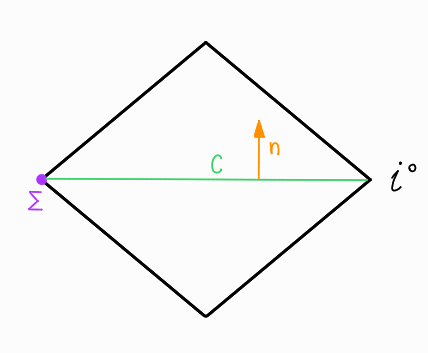
\includegraphics[width=6cm]{Capitulos/imagenes/fig1.png}
\centering
\caption{Diagrama de Penrose de la parte exterior de un agujero negro. Donde $i^{0}$ es el infinito espacial, $\Sigma$ corresponde a la superficie de bifurcación y $\mathcal{C}$ es la hipersuperficie de Cauchy.}
\end{figure}
Podemos ver que la hipersuperficie de Cauchy tiene borde interior $\Sigma$ y borde exterior $i^{0}$. Ahora, integraremos la variación de la corriente de Noether sobre $\mathcal{C}$. Luego, contrayendo con $\frac{1}{(D-2) !} \diff x^{\nu_2} \wedge \ldots \wedge \diff x^{\nu_D} $ e integrando sobre $\mathcal{C}$, tenemos 
\begin{align}\notag
\delta \int_\mathcal{C} \diff^{D-1} x \sqrt{|h|}n_\mu {\nabla_\nu q^{\mu \nu}}&=2 \int_\mathcal{C} \diff^{D-1} x \sqrt{|h|}n_\mu \nabla_\lambda(\xi^{[\lambda} \Theta^{\mu]})\\ \notag
\delta \int_\mathcal{C}\diff^{D-1}x \sqrt{|h|} D_\nu\left(n_\mu q^{\mu \nu}\right)&=2 \int_\mathcal{C} \diff^{D-1}x\sqrt{|h|} D_\nu\left(n_\mu \xi^{[\nu} \Theta^{\mu]}\right)\\ 
\delta \oint_{\partial\mathcal{C}} \diff^{D-2}x \sqrt{|\gamma|} u_\nu n_\mu q^{\mu \nu}&=2 \oint_{\partial \mathcal{C}} \diff ^{D-2}x \sqrt{|\gamma|} u_\nu n_\mu \xi^{[\nu} \Theta^{\mu]}\, ,
\end{align}
donde podemos observar que en la primera línea usamos que $J^{\mu}$ es una corriente conservada. Luego, en la segunda línea utilizamos que un vector normal contraído con un tensor antisimétrico puede ser escrito como la derivada $D$ de la multiplicación de dichos objetos y, como último paso, el teorema de la divergencia. A continuación si consideramos $\partial\mathcal{C}=\Sigma\cup i^{0}$ tenemos 
\begin{align}\notag
&\delta \int_{\infty} \diff^{D-2}x\sqrt{|\gamma|} u_\nu n_\mu q^{\mu \nu}-\delta \int_{\Sigma} \diff^{D-2}x\sqrt{|\gamma|} u_\nu n_\mu q^{\mu\nu}\\
&=2 \int_{\infty} \diff^{D-2}x\sqrt{|\gamma|} u_\nu n_\mu \xi^{[\nu} \Theta^{\mu]}-\cancelto{0}{{2 \int_{\Sigma} \diff^{D-2}x\sqrt{|\gamma|} u_\nu n_\mu \xi^{[\nu} \Theta^{\mu]}}} \, ,
\end{align}
en donde el último término se anula ya que el vector de Killing en el horizonte de bifurcación es cero y además, el signo menos viene de la orientación del vector normal. Así, nos queda 
\begin{align}\notag
\delta \int_{\infty}  \diff^{D-2}x\sqrt{|\gamma|} u_\nu n_\mu q^{\mu \nu} +2 \int_{\infty} d^{D-2}x \sqrt{\sigma} u_\nu n_\mu \xi^{[\nu} \Theta^{\mu]}=\delta \int_{\Sigma}  \diff^{D-2}x\sqrt{|\gamma|} u_\nu n_\mu q^{\mu\nu}\, .
\end{align}
Luego, recordando de la derivación del teorema de Noether, habíamos dicho que para tener una noción de energía debíamos considerar un termino de borde, así 
\begin{align}
\delta \int_{\infty}  \diff^{D-2}x\sqrt{|\gamma|} u_\nu n_\mu q^{\mu \nu} -2 \delta\int_{\infty} \xi^{\mu}\mathcal{B}^{\nu}\diff\Sigma_{\mu\nu} =\delta \int_{\Sigma}  \diff^{D-2}x\sqrt{|\gamma|} u_\nu n_\mu q^{\mu\nu}\, ,
\end{align}
 y con ello, todo lo que esta al lado izquierdo de la ecuación anterior es la variación de la energía, por tanto, nos queda 
 \begin{align}
\delta E =\delta \int_{\Sigma} \diff^{D-2}x\sqrt{|\gamma|} u_\nu n_\mu q^{\mu\nu}=\delta \int_{\Sigma} q^{\mu\nu} d\Sigma_{\mu\nu}\, .
 \end{align}
Del mismo modo, Wald en la Ref.~\cite{Wald:1993nt} identificó el lado derecho con $T\cdot S$ comparando con la primera ley de la termodinámica. Lo anterior esta justificado solamente si la temperatura se mantiene constante sobre la hipersuperficie de bifurcación. Asimismo, Iyer y Wald en la Ref.~\cite{Iyer:1994ys} demostraron como teorema lo siguiente 
\begin{align}
\delta \int_{\Sigma} q^{\mu\nu} d\Sigma_{\mu\nu}=\frac{k_s}{2\pi}\delta S \, ,
\end{align}
por lo que la Entropía del agujero negro es la carga de Noether en el horizonte, esto es, 
\begin{align}
S=\frac{1}{T} \int_{\Sigma} q^{\mu\nu} d\Sigma_{\mu\nu}\, . \label{entropy}
\end{align}









\subsection{Ejemplo: Relatividad General}
Ahora, consideremos el caso de Relatividad General y como solución a las ecuaciones de movimiento la métrica~\eqref{schw}. Sabemos que el Lagrangiano es de la siguiente manera
\begin{align}
    \Lag=\kappa R\equiv\kappa \delta^{[\lambda}_{[\mu}\delta^{\rho]}_{\nu]}R^{\mu\nu}_{\lambda\rho}\, .
\end{align}
Luego, de la definición de $E^{\lambda\rho}_{\mu\nu}$ 
\begin{align}
E^{\lambda\rho}_{\mu\nu}=\frac{\partial\Lag}{\partial R^{\mu\nu}_{\lambda \rho}}=\kappa \delta^{[\lambda}_{[\mu}\delta^{\rho]}_{\nu]}=\frac{\kappa}{2}\delta^{\lambda\rho}_{\mu\nu}\, .
\end{align}
Así, podemos calcular el prepotencial de Noether 
\begin{align}\notag
q^{\mu \nu} &=-2\left(E_{\lambda \rho}^{\mu \nu} \nabla^\lambda \xi^\rho+2 \xi^\lambda \nabla^\rho E_{\lambda \rho}^{\mu \nu}\right) \\ \notag
&=-2\left(\frac{\kappa }{2} \delta_{\lambda \rho}^{\mu \nu} \nabla^\lambda \xi^\rho\right) \\ \notag
&=-\kappa\left(\delta_\lambda^\mu \delta_\rho^\nu-\delta_\rho^\mu \delta_{\lambda}^\nu\right) \nabla^\lambda \xi^\rho \\ \notag
&=-\kappa\left(\nabla^\mu \xi^\nu-\nabla^\nu \xi^\mu\right)\\
&=-2\kappa\nabla^{[\mu}\xi^{\nu]} \, ,
\end{align}
entonces, la definición de energía para Relatividad General considerando que el termino de borde es $\mathcal{B}=2 \sigma \kappa (K-K_0)$ quedará
\begin{align}
H[\xi]=E=\kappa\int_{\infty}\left(-2\nabla^{[\mu}\xi^{\nu]}+4  \xi^{[\mu} n^{\nu]} \left[K-K_0\right]\right) \diff\Sigma_{\mu\nu}\, .
\end{align}
Los objetos de la integral son conocidos de las secciones anteriores. Así, calculando el primer término para un vector de Killing $\xi=\partial_{t}$, tenemos 
\begin{align}\notag
-\kappa\int_{\infty}2\nabla^{[\mu}\xi^{\nu]}\diff\Sigma_{\mu\nu}&=-2\kappa\sigma\int_{\infty}\diff^{2}x\,\sqrt{|\gamma|}\,\nabla_{\mu}\xi_{\nu}n^{[\mu}u^{\nu]}\\ \notag
&=-2\kappa\sigma\int_{\infty}\diff^{2}x\,\sqrt{|\gamma|}\,\nabla_{\mu}(g_{\nu\lambda}\xi_{\lambda})n^{[\mu}u^{\nu]}\\ \notag
&=-2\kappa\sigma\int_{\infty}\diff^{2}x\,\sqrt{|\gamma|}\,g_{\nu\lambda}\nabla_{\mu}\xi^{\lambda}n^{[\mu}u^{\nu]}\\ \notag
&=-2\kappa\sigma\int_{\infty}\diff^{2}x\,\sqrt{|\gamma|}\,g_{\nu\lambda}(\cancelto{0}{\partial_{\mu}\xi^{t}}+\Gamma^{\lambda}_{\mu\alpha}\xi^{\alpha})n^{[\mu}u^{\nu]}\\ \notag
&=-2\kappa\sigma\int_{\infty}\diff^{2}x\,\sqrt{|\gamma|}\,g_{\nu\lambda}(\Gamma^{\lambda}_{\mu t}\xi^{t})n^{[\mu}u^{\nu]}\\
&=-\cancel{2}\kappa\sigma\int_{\infty}\diff^{2}x\,\sqrt{|\gamma|}\,g_{\nu\lambda}(\Gamma^{\lambda}_{\mu t}\xi^{t})\left[\frac{1}{\cancel{2}}(n^{\mu}u^{\nu}-n^{\nu}u^{\mu})\right] \, .
\end{align}
Luego, los símbolos de Christoffel no nulos de la solución de Schwarzschild son
\begin{equation}
    \begin{array}{cc}
\Gamma^t_{rr} = \frac{GM}{r^2 f(r)} &
\Gamma^r_{tr} = \frac{GM}{r^2 f(r)} \\
\Gamma^r_{tt} = -\frac{GM}{r^2 f(r)} &
\Gamma^\theta_{\theta r} = rf(r) \\
\Gamma^\theta_{\phi\phi} = -\sin\theta\cos\theta &
\Gamma^\phi_{\theta\phi} = \frac{\cos\theta}{\sin\theta} \\
\Gamma^\phi_{\phi\theta} = \frac{\cos\theta}{\sin\theta} &
\Gamma^r_{rr} = \frac{GM}{r^2}\\
\Gamma^t_{tr} = \Gamma^t_{rt} = \frac{GM}{r^2} &
\Gamma^r_{\theta\theta} = -\frac{GM}{r^2}f(r) \\
\Gamma^r_{\phi\phi} = -r\sin^2\theta f(r) &
\Gamma^t_{\theta\theta} = rf(r) \\
\Gamma^t_{\phi\phi} = -r\sin^2\theta f(r) &
\Gamma^\theta_{r\theta} = \Gamma^\theta_{\theta r} \\
\Gamma^\phi_{r\phi} = \Gamma^\phi_{\phi r} = \frac{1}{r}f(r) &
\end{array}
\end{equation}


Luego, remplanzando los valores de los Christoffel, obtenemos
\begin{align}\notag
-\kappa\int_{\infty}2\nabla^{[\mu}\xi^{\nu]}\diff\Sigma_{\mu\nu}&=-\kappa\sigma\int_{0}^{\pi}\int_{0}^{2\pi}\diff\theta \diff\phi\,\left(g_{tt}\frac{1}{2f(r)}f'(r)-g_{rr}\frac{1}{2}f(r)f'(r)\right)r^{2}\sin{\theta}\\ \notag
&=-\kappa\sigma\int_{0}^{\pi}\int_{0}^{2\pi}\diff\theta \diff\phi\,\left(-\cancel{f(r)}\frac{1}{2\cancel{f(r)}}f'(r)-\frac{1}{\cancel{f(r)}}\frac{1}{2}\cancel{f(r)}f'(r)\right)r^{2}\sin{\theta} \\ \notag
&=-\kappa\sigma\int_{0}^{\pi}\int_{0}^{2\pi}\diff\theta \diff\phi\,\left[f'(r)\right]r^{2}\sin{\theta} \notag \, .
\end{align}
Así, integrando y remplazando el valor de $\kappa$, nos queda
\begin{align}
-\kappa\int_{\infty}2\nabla^{[\mu}\xi^{\nu]}\diff\Sigma_{\mu\nu}=\frac{m}{2}\, .
\end{align}
Ahora, el segundo término es
\begin{align}\notag
\kappa\int_{\infty}4  \xi^{[\mu} n^{\nu]} \left[K-K_0\right]\diff\Sigma_{\mu\nu}&=4\kappa\sigma\int_{\infty}\sqrt{|\gamma|}\,\cancel{\sqrt{f(r)}}\left[\frac{f'(r)+4f(r)-4\sqrt{f(r)}}{2r\cancel{\sqrt{f(r)}}}\right]n_{[t}u_{r]}\diff^{2}x\\ \notag
&=4\kappa\sigma\int_{\infty}\sqrt{|\gamma|}\,\left[\frac{f'(r)+4f(r)-4\sqrt{f(r)}}{2r}\right]\frac{1}{2}(\cancel{n_{t}u_{r}}-n_{r}u_{t})\diff^{2}x\\ \notag
&=2\kappa\sigma\int_{\infty}\sqrt{|\gamma|}\,\left[\frac{f'(r)+4f(r)-4\sqrt{f(r)}}{2r}\right][-f(r)]\diff^{2}x\\ \notag
&=2\kappa\sigma\int_{0}^{\pi}\int_{0}^{2\pi}\diff\theta \diff\phi\,\left[\frac{f'(r)+4f(r)-4\sqrt{f(r)}}{2\cancel{r}}\right][-f(r)]r^{\cancel{2}}\sin{\theta}\, .
\end{align}
Entonces, sustiyuyendo el valor de $f(r)$ e integrando, obtenemos 
\begin{align}
    \kappa\int_{\infty}4  \xi^{[\mu} n^{\nu]} \left[K-K_0\right]\diff\Sigma_{\mu\nu}=\frac{m}{2}\, .
\end{align}
Finalmente, el valor de la energía será 
\begin{align}
H[\xi]=E=\kappa\int_{\infty}\left(-2\nabla^{[\mu}\xi^{\nu]}+4  \xi^{[\mu} n^{\nu]} \left[K-K_0\right]\right) \diff\Sigma_{\mu\nu}=\frac{m}{2}+\frac{m}{2}=m\, ,
\end{align}
lo cual concuerda con los métodos usados anteriormente y adicionalmente es el valor esperado al calcular una cantidad conservada asociada a una simetría temporal.

Por otro lado, para obtener la temperatura $T$ de la Ec.~\eqref{temp}, debemos calcular la gravedad superficial. Entonces usando~\eqref{surfgrav2} 
\begin{align} \notag
\kappa^{2}_{s}&=-\frac{1}{2}(\nabla_{\mu}\xi_{\nu})(\nabla^{\mu}\xi^{\nu})\\ \notag
&=-\frac{1}{2}\left[\nabla_{\mu}(g_{\nu\lambda}\xi^{\lambda})(g^{\mu\alpha}\nabla_{\alpha}\xi^{\nu})\right]\\ \notag
&=-\frac{1}{2}g_{\nu\lambda}(\cancelto{0}{\partial_{\mu}}\xi^{\lambda}+\Gamma^{\lambda}_{\beta\mu}\xi^{\beta})g^{\mu\alpha}(\cancelto{0}{\partial_{\alpha}}\xi^{\nu}+\Gamma^{\nu}_{\sigma\alpha}\xi^{\sigma})\\ \notag
&=-\frac{1}{2}(g_{\nu\lambda}\Gamma^{\lambda}_{\beta\mu}\xi^{\beta})(g^{\mu\alpha}\Gamma^{\nu}_{\sigma\alpha}\xi^{\sigma})\\ \notag
&=-\frac{1}{2}(g_{\nu\lambda}\Gamma^{\lambda}_{t\mu}\xi^{t}g^{\mu\alpha}\Gamma^{\nu}_{t\alpha}\xi^{t})\\ \notag
&=-\frac{1}{2}g^{\mu\alpha}(g_{tt}\Gamma^{t}_{\mu t}\Gamma^{t}_{\alpha t}+g_{rr}\Gamma^{r}_{\mu t}\Gamma^{r}_{\alpha t})\\ \notag
&=-\frac{1}{2}(g^{rr}g_{tt}\Gamma^{t}_{rt}\Gamma^{t}_{rt}+g^{tt}g_{rr}\Gamma^{r}_{tt}\Gamma^{r}_{tt})\\ \notag
&=-\frac{1}{2}\left(\frac{-1}{4}\cancel{f^{2}(r_{h})}f'^{2}(r_{h})\frac{1}{\cancel{f^{2}(r_{h})}}-\frac{1}{4}\frac{1}{\cancel{f^{2}(r_{h})}}f'^{2}(r_{h})\cancel{f^{2}(r_{h})}\right)\\ 
&=\frac{1}{4}f'^{2}(r_{h})\, .
\end{align}
Tomando raíz cuadrada a ambos lados nos queda 
\begin{align}
    \kappa_{s}=\frac{mG}{r^2_{h}}\, .
\end{align}
Además, dada la definición de horizonte podemos despejar $m$ en función de $r_h$ y viceversa 
\begin{align}
    f_{r_h}=0 \to r_{h}=2mG\, ,
\end{align}
entonces, tenemos
\begin{align}
    \kappa_{s}=\frac{mG}{4m^2 G^2}=\frac{1}{4mG}\, .
\end{align}
Finalmente, usando la Ec.~\eqref{temp} obtenemos el valor de la temperatura
\begin{align}
    T=\frac{\kappa_{s}}{2\pi}=\frac{1}{8\pi mG}\, . \label{temp2}
\end{align}

Ahora bien, con el prepotencial también podemos calcular la entropía para la solución~\eqref{schw}. Usando~\eqref{entropy} tenemos
\begin{align}\notag
TS&=-2\kappa\int_{\Sigma}\sqrt{|\gamma|}\nabla^{[\mu}\xi^{\nu]}n_{[\mu}u_{\nu]}\diff^{2}x\\ \notag
&=-2\kappa\int_{\Sigma}\sqrt{|\gamma|}\nabla_{\mu}\xi_{\nu}n^{[\mu}u^{\nu]}\diff^{2}x\\ \notag
&=-2\kappa\int_{\Sigma}\sqrt{|\gamma|}g_{\mu\lambda}\nabla_{\mu}\xi^{\lambda}n^{[\mu}u^{\nu]}\diff^{2}x\\ \notag
&=-2\kappa\int_{\infty}\sqrt{|\gamma|}\,g_{\nu\lambda}(\cancelto{0}{\partial_{\mu}\xi^{t}}+\Gamma^{\lambda}_{\mu\alpha}\xi^{\alpha})n^{[\mu}u^{\nu]}\,\diff^{2}x\\ \notag
&=-2\kappa\int_{\infty}\sqrt{|\gamma|}\,g_{\nu\lambda}(\Gamma^{\lambda}_{\mu t}\xi^{t})n^{[\mu}u^{\nu]}\,\diff^{2}x\\ \notag
&=-\cancel{2}\kappa\int_{\infty}\sqrt{|\gamma|}\,g_{\nu\lambda}(\Gamma^{\lambda}_{\mu t}\xi^{t})\left[\frac{1}{\cancel{2}}(n^{\mu}u^{\nu}-n^{\nu}u^{\mu})\right]\,\diff^{2}x \\ \notag
&=-\kappa\int_{0}^{\pi}\int_{0}^{2\pi}\diff\theta \diff\phi\,\left(g_{tt}\frac{1}{2f(r)}f'(r)-g_{rr}\frac{1}{2}f(r)f'(r)\right)r^{2}\sin{\theta}\\ \notag
&=-\kappa\int_{0}^{\pi}\int_{0}^{2\pi}\diff\theta \diff\phi\,\left(-\cancel{f(r)}\frac{1}{2\cancel{f(r)}}f'(r)-\frac{1}{\cancel{f(r)}}\frac{1}{2}\cancel{f(r)}f'(r)\right)r^{2}\sin{\theta} \\ 
&=-\kappa\int_{0}^{\pi}\int_{0}^{2\pi}\diff\theta \diff\phi\,\left[f'(r)\right]r^{2}\sin{\theta}=\frac{m}{2}  \, .
\end{align}
Luego, para el horizonte $r=r_{h}=2mG$ podemos escribir en función de $r_{h}$, siendo $m=r_{h}/2G$. Además, usando la Ec.~\eqref{temp2} y que $A=4\pi r^{2}_{h}$, nos queda 
\begin{align} \notag
S&=8\pi G \frac{m^{2}}{2}\\ \notag
    &=4\pi G \frac{r^{2}_{h}}{4G^2}\\
    &=\frac{r^{2}_{h}\pi}{G}\, ,
\end{align}
Lo cual es equivalente a 
\begin{align}
    S=\frac{r^{2}_{h}\pi}{G}=\frac{A}{4G}\, .
\end{align}
Es decir,la entropía satisface la ley de un cuarto del área. Además, estas cantidades satisfacen la primera ley de la termodinámica, $\delta M=T\delta S$










\section{Acción Euclídea on-shell \label{sec:AEO}}
Finalmente, revisaremos un formalismo para calcular cantidades conservadas que guarda estrecha relación con las leyes de la termodinámica. Con el fin de usar este método, es necesario tener un principio variacional bien definido. Por lo tanto, aún es necesaria la adición de un termino de borde~\cite{Gibbons:1976ue}. En el caso de Relatividad General, ya vimos que es suficiente sumar la curvatura extrínseca de la variedad para imponer condiciones de borde tipo Dirichlet. 

Consideremos nuevamente la métrica de Schwarzschild en 4 dimensiones dada por la Ec.~\eqref{schw} y apliquemos la rotación de Wick $t\to -i\tau$, lo que nos entrega
\begin{align}
 \diff s^2=\left(1-\frac{2mG}{r}\right)\diff \tau^2+\frac{\diff r^2}{\left(1-\frac{2mG}{r}\right)}+r^2\left(\diff \theta^2+\sin^2\theta\diff \phi^2\right) \, . \label{euclids}
\end{align}
Ahora, el elemento de línea tiene signatura Euclídea, por lo que $f(r)\geq 0$. Este cambio de signo podría inducir singularidades en la variedad, por lo que vamos a revisar con detalles el rango de $\tau$. 

Analicemos la geometría descrita por esta métrica cerca del horizonte $r=r_h$, en donde $f(r_h)=0$. Expandiendo $f(r)$ en torno al horizonte, obtenemos
\begin{align}
    f(r)=\cancelto{0}{f(r_h)}+f'(r)(r-r_h)+\cdots
\end{align}
donde el primer término es cero dado que es la definición de horizonte. Así, el elemento de linea se verá como 
\begin{align}
    \diff s^2\approx f'(r_h)(r-r_h)\diff \tau^2+\frac{\diff r^2}{f'(r)(r-r_h)}+r_h^2\left(\diff \theta^2+\sin^2\theta\diff \phi^2\right)\, .
\end{align}
A continuación, haremos el siguiente cambio de coordenadas
\begin{align}
    \diff\rho^2=\frac{\diff r^2}{f'(r_h)(r-r_h)}\;\;\;\;\;\mbox{o bien}\;\;\;\;\; r-r_h=\frac{\rho^2 f'^2(r_h)}{4}\, ,
\end{align}
lo que nos entrega
\begin{align}
    \diff s^2\approx\frac{\rho^2 f'^2(r_h)}{4}\diff\tau^2+\diff\rho^2+r_h^2\left(\diff \theta^2+\sin\theta\diff \phi^2\right)\, .
\end{align}
Luego, es posible definir una nueva variable angular, en particular 
\begin{align}
    \psi\equiv\frac{f'(r_h)}{2}\tau \;\;\;\to\;\;\; \diff\psi^2=\frac{f'^2(r_h)}{4}\diff\tau^2 \, .
\end{align}
De este modo, la métrica de Schwarzschild cerca del horizonte se ve 
\begin{align}
    \diff s^2\approx\rho^2\diff\psi^2+\diff\rho^2+r_h^2\left(\diff \theta^2+\sin^2\theta\diff \phi^2\right)\, . \label{euclideo}
\end{align}
Como habíamos mencionado anteriormente, queremos evitar singularidades. En este caso, para evitar singularidades cónicas, vamos a pedir que el periodo de la nueva variable sea $\psi\sim\psi +2\pi$, lo que implica que $\tau\sim\tau+\beta_{\tau}$, en donde 
\begin{align}
    \beta_{\tau}=\frac{4\pi}{f'(r_h)}\, , \label{btau}
\end{align}
es el período del tiempo Euclídeo. De esta forma, el rango de las coordenadas de la métrica~\eqref{euclideo} es $0\leqslant\tau\leqslant\beta_{\tau}$, $r_{h}\leqslant r<\infty$, $0\leqslant\theta\leqslant\pi$ y $0\leqslant\phi\leqslant 2\pi$, lo cual garantiza que es completamente regular. De hecho, podemos notar que las hipersuperficies de $\rho$ constante son topológicamente $\mathbb{S}^1\times\mathbb{S}^2$. 

Luego de que nos hemos asegurado que la métrica esta libre de singularidades, la mecánica estadística nos permite relacionar el período del tiempo Euclídeo con el inverso de la temperatura, esto es, $\beta_{\tau}=T_{H}^{-1}$, en donde $T_H$ es la temperatura de Hawking del agujero negro. De hecho, esta cantidad coincide con la obtenida a través de la gravedad superficial, la cual se define como~\eqref{surfgrav2}.
En el caso de la métrica de Schwarzschild encontramos
\begin{align}
    T_{H}=\frac{1}{8\pi mG} \, .
\end{align}
Éste resultado nos será de utilidad para el cálculo de la termodinámica del agujero negro a partir de la relación entre la función partición y la acción Euclídea on-shell. Esta relación la obtendremos mediante el procedimiento que es mostrado a continuación. 




\subsection{Aproximación de punto silla}
Consideremos la siguiente integral
\begin{align}
    I=\int^{\infty}_{-\infty}\diff x \, \,e^{-f(x)}\, ,
\end{align}
en donde $f(x):\mathbb{R}\to\mathbb{R}$ y sea $x=x_{0}$ un extremo de la función, i.e., 
\begin{align}
    f'(x)\big|_{x=x_{0}}=0\, .
\end{align}
Expandiendo $f(x)$ en torno a este punto, tenemos
\begin{align}
    f(x)=f(x_{0})+\cancelto{0}{f'(x_{0})(x-x_{0})}+\frac{1}{2}f''(x_{0})(x-x_{0})^{2}+\cdots \, .
\end{align}
De este modo, a segundo orden en la expansión, la integral queda
\begin{align}\notag
I&\approx\int^{\infty}_{-\infty}\diff x \, \,e^{-f(x_{0})-\frac{1}{2}f''(x_{0})(x-x_{0})^{2}}\\
&\approx e^{-f(x_{0})}\int^{\infty}_{-\infty}\diff x \, \,e^{-\frac{1}{2}f''(x_{0})(x-x_{0})^{2}} \label{gauss}\, ,
\end{align}
en donde hemos utilizado que la primera integral es una constante. Luego, para que la integral no sea divergente, debemos pedir que $f''(x_{0})>0$. Esto implica que $x_0$ es un mínimo de $f(x)$. De este modo, la Ec.~\eqref{gauss} es una Gaussiana y, por lo tanto, tiene un resultado conocido que es
\begin{align}
    I\approx e^{-f(x_{0})}\int^{\infty}_{-\infty}\diff x \, \,e^{-\frac{1}{2}f''(x_{0})(x-x_{0})^{2}}= e^{-f(x_{0})}\sqrt{\frac{2\pi}{f''(x_{0})}}\, .
\end{align}
A este procedimiento se le conoce como aproximación de punto silla. 

\subsection{Función partición para una solución asintóticamente plana} \label{funcionparticion}

Tomando en cuenta el resultado de la subseccion anterior, consideremos la función partición de un sistema escrito en el formalismo de integral de camino de la mecánica cuántica
\begin{align}
     \mathcal{Z}=\int \mathcal{D}\phi \,\, e^{i\int \diff^4 x \sqrt{\lvert g \lvert} \;\Lag[\phi]}\, ,\label{funcionp}
\end{align}
en donde $\int \mathcal{D}\phi$ es la integral sobre todas las configuraciones de campo $\phi$. Realicemos una rotación de Wick $t\to -i\tau$ de modo que el elemento de volumen transforma como $\diff^4 x \sqrt{\lvert g \lvert}\to -i\diff^4 x_{E}\sqrt{\lvert g_{E} \lvert}$, en donde $E$ denota cantidades definidas en el espacio Euclídeo. Así, la integral~\eqref{funcionp} se verá como
\begin{align}
    \mathcal{Z}=\int \mathcal{D}\phi \,\, e^{\int \diff^4 x_{E} \sqrt{\lvert g_{E} \lvert} \;\Lag[\phi_{E}]}\equiv\int \mathcal{D}\phi \,\, e^{-I^{\rm E}_{\rm cl}[\phi]}\, ,
\end{align}
con $I^{\rm E}_{\rm cl}[\phi]$ siendo la acción Euclídea clásica. Usemos la aproximación de punto silla para encontrar la función partición. Consideremos una configuración que minimice la acción Euclídea, por ejemplo, una solución a las ecuaciones de movimiento que denotaremos por $\phi=\phi_{0}$. Expandiendo la acción en torno a esta configuración obtenemos  
\begin{align}
    I^{\rm E}_{\rm cl}[\phi]&=I^{\rm E}_{\rm cl}[\phi_{0}]+\cancelto{0}{\frac{\delta I^{\rm E}_{\rm cl}}{\delta\phi}\big|_{\phi=\phi_{0}}(\phi-\phi_{0})}+\frac{1}{2}\frac{\delta^{2} I^{\rm E}_{\rm cl}}{\delta\phi^{2}}\big|_{\phi=\phi_{0}}(\phi-\phi_{0})^{2}+\cdots\, ,
\end{align}
en este caso el segundo término se anula dado que la variación funcional de la acción con respecto a los campos son las ecuaciones de movimiento, por lo tanto, son cero evaluadas en una solución. Luego, la función partición queda 
\begin{align}
    \mathcal{Z}&\approx \int \mathcal{D}\phi \,\, e^{-I^{\rm E}_{\rm cl}[\phi_{0}]-\frac{1}{2}\frac{\delta^{2} I^{\rm E}_{\rm cl}}{\delta\phi^{2}}\big|_{\phi=\phi_{0}}(\phi-\phi_{0})^{2}}=C\, e^{-I^{\rm E}_{\rm cl}[\phi_{0}]}\, ,
\end{align}
en donde $C$ es una constante que sin perdida de generalidad puede ser fijada a 1. Entonces, tomando el logaritmo en ambos lados de la ecuación anterior, llegamos a la siguiente expresión 
\begin{equation}
 \ln \mathcal{Z} \approx -I^{\rm E}_{\rm cl}[\phi_{0}]\, .
\end{equation}
A partir de esta relación, es posible obtener las cantidades termodinámicas del sistema usando las relaciones de la mecánica estadística. Por ejemplo, la energía libre, la energía interna y la entropía se pueden obtener de
\begin{align}\label{free}
    F&=-T\ln\mathcal{Z}\approx\beta^{-1}I^{\rm E}_{\rm cl}\, ,\\ 
    U&=-\frac{\partial}{\partial\beta}\ln\mathcal{Z}\approx\frac{\partial}{\partial\beta}I^{\rm E}_{\rm cl} \label{internal}\, ,\\ 
    S&=\beta U+\ln\mathcal{Z}\approx\left(\beta\frac{\partial}{\partial\beta}-1\right)I^{\rm E}_{\rm cl}\label{entropy1}\, ,
\end{align}
respectivamente. Estas relaciones son de gran utilidad para derivar las leyes de la termodinámica de los agujeros negros tal como se mostró en la Ref.~\cite{Gibbons:1976ue}.

Evaluemos la acción Euclídea on-shell para la solución~\eqref{euclids}. Primero, podemos ver que dicha métrica es solución de $R_{\mu\nu}=0$, lo cual implica $R=0$. Así, observamos que el término de volumen de la acción~\eqref{acciondir} se anula, dando como resultado solamente el término de borde on-shell, esto es,
\begin{align}
    I^{\rm E}_{\rm cl}=-2\kappa\int \diff^3 x \sqrt{\lvert h_E \rvert}\, (K-K_0)\, . \label{aeosch}
\end{align}
Aquí, hemos elegido una foliación radial, cuyo  vector normal unitario a las hipersuperficies con $r$ constante es $n=n^{\mu}\partial_\mu=\sqrt{f(r)}\partial_r$. Los valores de $K$ y $K_0$ ya los obtuvimos cuando calculamos la carga con el método de Brown-York, siendo estos
\begin{align}
    K&=\frac{f'(r)r+4f(r)}{2r\sqrt{f(r)}}\, \label{curvextri},\\
    K_0&=\frac{2}{r}\, ,
\end{align}
para Schwarzschild (con $f(r)=1-2mG/r$) y  Minkowski, respectivamente. Antes de evaluar la acción, debemos considerar que ambas métricas deben estar en el mismo ensamble a temperatura fija. Dicha condición se traduce a que ambos elementos de línea deben tener las mismas condiciones de borde. Con el fin de conseguir esto, debemos asegurarnos que las longitudes de arco de ambas métricas coincidan para toda hipersuperficie de $r$ constante. En este punto, podemos fijar $\theta$ y $\phi$ sin pérdida de generalidad, ya que $h_{\theta\theta}$ y $h_{\phi\phi}$ coinciden con $h^{(0)}_{\theta\theta}$ y $h^{(0)}_{\phi\phi}$; no así $h_{\tau\tau}$ con $h^{(0)}_{\tau\tau}$, donde $h^{(0)}_{\mu\nu}$ es la métrica inducida del background a $r$ constante. Pedir esta condición se visualiza de la siguiente manera 
\begin{align}\notag
\int \sqrt{\diff s^2}\big|_{r=R}&=\int \sqrt{\diff s^2_{(0)}}\big|_{r=R}\\ \notag
\int_{0}^{\beta_\tau}\sqrt{f(R)}\diff\tau&=\int_{0}^{\beta_0}\diff\tau\\
\beta_\tau\sqrt{f(R)}&=\beta_0 \label{periodo}\,
\end{align}
Esta condición fija $\beta_0$ en función de $\beta_\tau$. Con esto en mente, evaluemos la acción Euclídea on-shell~\eqref{aeosch}
\begin{align}\notag
I^{\rm E}_{\rm cl}&=-2\kappa\int \diff^3 x \sqrt{\lvert h_E \rvert}\, (K-K_0)\\ \notag
&=-2\kappa\int^{2\pi}_{0}\diff\phi\int^{\pi}_{0}\diff\theta\sin\theta\int^{\beta_\tau}_{0}\diff\tau\left[\sqrt{f(r)}r^2\left(\frac{f'(r)r+4f(r)}{2r\sqrt{f(r)}}-\frac{2}{r}\right)\right]\\ \notag
&=-8\pi\kappa\int^{\beta_\tau}_{0}\diff\tau\left(\frac{r^{2}f'(r)+4f(r)r}{2}-2\sqrt{f(r)}r\right)\\ \notag
&=-8\pi\kappa\int^{\beta_\tau}_{0}\diff\tau\left(mG+2r-4mG-2r\sqrt{1-\frac{2mG}{r}}\right)\\ \notag
&=-8\pi\kappa\int^{\beta_\tau}_{0}\diff\tau\left(mG+2r-4mG-2r\left\{1-\frac{1}{2}\left(\frac{2mG}{r}\right)-\mathcal{O}(r^{-2})\right\}\right)\\ \notag
&=8\pi\kappa\beta_\tau mG\\
 &=\frac{1}{2}\beta_\tau m\, ,
\end{align}
donde en el último paso reemplazamos el valor de $\kappa$. De la definición de horizonte y de la Ec.~\eqref{btau} podemos reescribir el resultado anterior en función del radio de Schwarzschild $r_h$, quedando
\begin{align}
    I^{\rm E}_{\rm cl}=\frac{1}{2}4\pi r_h\frac{r_h}{2G}=\frac{\pi r_{h}^2}{G}\, .
\end{align}
Luego, podemos calcular las cantidades termodinámicas de las Ecs.~\eqref{free},~\eqref{internal} y~\eqref{entropy1} , obteniendo así 
\begin{align}
    F&\approx\beta^{-1}I^{\rm E}_{\rm cl}=\frac{r_h}{4G}\, ,\\ 
    U&\approx\frac{\partial}{\partial\beta}I^{\rm E}_{\rm cl} =M\, ,\\ 
    S&\approx\left(\beta\frac{\partial}{\partial\beta}-1\right)I^{\rm E}_{\rm cl}=\frac{\pi r_{h}^2}{G}\, .
\end{align}
Vale la pena destacar que la entropía cumple con la ley del cuarto del área de la fórmula de Bekenstein-Hawking. Además, la energía interna coincide con el valor de la masa del agujero negro.

En síntesis, en este capítulo revisamos en la teoría de relatividad general, su principio variacional y distintos métodos para calcular cargas conservadas para una solución asintoticamente plana. Si bien, hemos obtenido resultados correctos y compatibles con la teoría veremos en los capítulos que siguen que al tratar con soluciones con distinta asíntota los métodos ya mencionados fallan y es necesaria una nueva prescripción para el cálculo de las cargas. Además, como estamos interesados en una teoría que está acoplada con materia vamos a añadir campos escalares y estudiar como se comporta dicha acción e introducir un nuevo método de renormalizacion que se basa en las simetrías de ésta.










\biblio %Se necesita para referenciar cuando se compilan subarchivos individuales - NO SACAR
\end{document}